\documentclass[12pt,a4paper,automark, toc=bib]{scrreprt}
\linespread{1.2}
%Sprache
\usepackage[utf8]{inputenc}
\usepackage{titling}
\usepackage{comment}
\usepackage[english]{babel}
\usepackage[T1]{fontenc}
\usepackage{dirtytalk}
%Mathe
\usepackage{nth}
%Format
\usepackage{times}
\usepackage{amsmath}
\usepackage{amsfonts}
\usepackage{amssymb}
\usepackage{etoc}
\usepackage{lipsum}
\usepackage[headsepline]{scrlayer-scrpage}
\usepackage{pdfpages}
\usepackage{geometry}
\usepackage{array}
\usepackage{subcaption}
\usepackage{algorithm}
\usepackage{algpseudocode}
\usepackage{booktabs}
\usepackage{siunitx}
\usepackage{collcell}
\usepackage{xstring}
\usepackage{tikz}
\usepackage{xcolor}
\usepackage[defaultlines=4,all]{nowidow}


\newcommand*{\MinNumber}{0}%
\newcommand*{\MidNumber}{50} %
\newcommand*{\MaxNumber}{100}%
\newcommand{\ApplyGradient}[1]{%
	\IfDecimal{#1}{%
		\ifdim #1 pt > \MidNumber pt%
		\pgfmathsetmacro{\PercentColor}{max(min(100.0*(#1 - \MidNumber)/(\MaxNumber-\MidNumber),100.0),0.00)} %
		\hspace{1pt}\colorbox{green!\PercentColor!white}{#1}%
		\else%
		\pgfmathsetmacro{\PercentColor}{max(min(100.0*(\MidNumber - #1)/(\MidNumber-\MinNumber),100.0),0.00)} %
		\hspace{1pt}\colorbox{magenta!\PercentColor!white}{#1}%
		\fi%
	}{#1}
}

\newcolumntype{R}{>{\collectcell\ApplyGradient}c<{\endcollectcell}}

\DeclareMathOperator*{\argmax}{arg\,max}

%Bibliographie
\usepackage[
backend=biber,
style=ieee,
sorting=nyt
]{biblatex}
\addbibresource{library.bib}

\usepackage{amsthm}
\theoremstyle{definition}
\newtheorem{definition}{Definition}[chapter]

% Page geometry
\geometry{
	left=25mm,
	right=2cm,
	top=20mm,
	bottom=20mm,
	footskip=10mm
}
\raggedbottom
\addtolength{\topskip}{0pt plus 10pt}



%Metadata for Title
\author{Jeff Schymiczek}
\title{Detection of Computationally Intensive Reversible Covert Channels with Shape Analysis of Empirical Probability Distributions}
\subject{Applied Computer Science}
\date{June 2022}



%header & footer
\clearpairofpagestyles
\setkomafont{pageheadfoot}{\normalfont}

\makeatletter
\let\inserttitle\@title
\makeatother

\newpairofpagestyles{normalpage}{
	\ihead{Jeff Schymiczek}
	\ohead{\pagemark}
	\chead{\headmark}
	\cfoot{\scriptsize{\inserttitle}}
}

\newpairofpagestyles{chapter}{
	\ihead{Jeff Schymiczek}
	\ohead{\pagemark}
	\cfoot{\scriptsize{\inserttitle}}
}

\newpairofpagestyles{title}{
	\ihead{
\includegraphics{figures/FH_Worms.png}}
}

\renewcommand{\chapterpagestyle}{chapter}
\renewcommand{\titlepagestyle}{title}
\pagestyle{normalpage}


%-------------------------------------------------------------
%							Document
%-------------------------------------------------------------

\begin{document}
	\pagenumbering{roman}
	\begin{titlepage}
		\centering
		\vfill
		{\bfseries
			\Large
			University of Applied Sciences Worms \\
			\large
			Department of Computer Science\\
			Applied Computer Science B.Sc.
			\vskip1cm
			\huge
			\inserttitle \\
			\vskip1cm
			\normalsize
		}
		Thesis in Fulfilment of the Requirements for the Degree of \\
		\Large
		\textbf{Bachelor of Science}\\
		\normalsize
		\vskip1cm
		Submitted by \\
		\Large
		\textbf{Jeff Schymiczek} \\
		\vskip2cm
		  	
		 \normalsize
		\vfill
		
\includegraphics[width=6cm]{figures/FH_Worms.png}
		\vfill
		\begin{center}
		\begin{tabular}[H]{ll}
			Matrikelnummer: & 674206\\
			Gutachter: & Prof. Dr. Steffen Wendzel\\
			Zweitgutachter: & Prof. Dr. Ralf Keidel \\
			Weitere Betreuende: & Tobias Schmidbauer\\
			Bearbeitungszeitraum: & Sommersemester 2022 \\
			Abgabedatum: & 30. Juni 2022 \\
			Sperrvermerk: & Nein
		\end{tabular}
		\end{center}
		\vfill
		\vfill
	\end{titlepage}

	\begin{abstract}
		
		\begin{center}
			{\textbf{Abstract}}
			\vskip2em
			
		\end{center}
	
	\textit{(English)}
	Reversible covert channels are a novel type of network security threat that make use of noise free covert storage channels, but restore the carrier packet before sending it to the overt receiver. This thesis proposes ways of utilizing runtime distribution shape analysis, a technique that has already shown success for the detection of timing channels, in order to recognize computationally intensive reversible covert channels. We simulated the latency of traffic modified by a hash-chain based covert channel by adding mock hash-reconstruction runtimes to measurements of legitimate ping traffic. After qualitatively observing the changes that occur in the empirical probability distribution and several statistical metrics between modified and natural traffic, we investigated machine learning algorithms for their ability to detect the covert channel's presence. We can report a that a decision tree based AdaBoost classifier using the investigated statistical measures as input vector and a convolutional neural network applied directly to the packet runtime empirical probability distribution are able to classify sets of 50 ping measurements with very high accuracy for low to medium high latency connections. Compared with previous work done on the investigated covert channel using mean-threshold tests, our approach both requires smaller sampling window sizes and achieves higher accuracy on the same reference dataset.
	\\
	\vskip2em
	\textit{(Deutsch)}
	Reversible verdeckte Kanäle sind eine neuartige Netzwerksicherheitsbedrohung, die auf rauschfreien Covert Storage Channels basieren, aber die Trägernachricht wiederherstellen, bevor sie an den eigentlichen Empfänger weitergeleitet wird. In dieser Arbeit demonstrieren wir, dass eine Formanalyse der empirischen Wahrscheinlichkeitsverteilung von Packetlaufzeiten zur Erkennung dieser Kanäle genutzt werden kann. Diese Technik hat sich bereits bei der Erkennung von Covert Timing Channels als erfolgreich erwiesen. Wir simulieren die Latenzzeit eines Netz\-werkverkehrs, der durch einen auf Hash-Ketten basierenden verdeckten Kanal verändert wurde, indem wir auf legitime Ping-Messungen simulierte Hash-Rekonstruktionszeiten aufaddieren. Veränderungen in der empirischen Wahrscheinlichkeitsverteilung und verschiedenen statistischen Metri\-ken zwischen modifiziertem und natürlichem Verkehr werden qualitativ erfasst und für ihre Verwendung in statistischen Entscheidungsmodellen bewertet. Wir können berichten, dass ein auf Entscheidungsbäumen basierender AdaBoost-Algorithmus mit den untersuchten statistischen Maß\-en als Eingangsvektor und ein direkt auf die empirische Wahrscheinlichkeitsverteilung angewandtes Convolutional Neural Network in der Lage sind, Sätze von 50 Ping-Messungen mit sehr hoher Genauig\-keit für Verbindungen mit niedriger bis mittlerer Latenz zu klassifizieren. Im Vergleich zu früheren Arbeiten zum untersuchten verdeckten Kanal, bei denen Schwellwerttests zur Erkennung des verdeckten Kanals verwendet wurden, erfordert unser Ansatz für denselben Datensatz eine kleinere Menge an Messungen und kann eine höhere Genauigkeit erzielen.
		
		
		
	\end{abstract}
	\tableofcontents	
	\listoffigures
	\listoftables
	
	%---------------------------------------------------------
	%						Introduction
	%---------------------------------------------------------
	
	
	\chapter{Introduction}
		\pagenumbering{arabic}
		
		Covert channels represent serious breaches of network security policy that can be used to  undermine the confidentiality of user data by enabling the communication of processes with conflicting privileges. They provide a way for malicious individuals or processes to communicate without record of their communication existing. Thusly they shield data leakage, botnet coordination and other harmful activities from detection. The ability to transfer illicit information unnoticed can however also be used for good, e. g. to enable whistleblowers and to subvert government censorship  \cite{Wendzel2015}. \\
		Recently reversible covert channel, i. e. such that reconstruct the original carrier data after completing the covert information transfer, came under increased scrutiny  \cite{Mazurczyk2019}. Because the received data remains unchanged, the overt receiver can only detect the channel's presence by observing network characteristics. The simplest such network characteristic is latency. An increase of which would be especially noticeable for computationally intensive channels. One such channel using TCP hash-chains has been theorised and investigated in  \cite{Keller2021}. Further research by Schmidbauer and Wendzel  \cite{Schmidbauer2021, Schmidbauer} established the possibility of its detection through the observation of increased packet runtimes.\\
		This thesis aims to build on the work of Schmidbauer and Wendzel by analysing not just the sum total of packet runtimes but their distribution. Shape analysis of packet runtime empirical probability distributions plays an important part in detecting covert channels of the inter-arrival pattern  \cite{Berk2005, Cabuk2009}. We propose the application of similar techniques to detect computationally intensive covert channels. Our goal is to qualitatively describe characteristics of the empirical probability distributions of overt and covert network traffic that would enable their differentiation. Based on these observations, statistical models are quantitatively investigated in order to establish robust methods of distinction. \\
		We reiterate and confirm the literature consensus that network traffic runtime possesses a asymmetrical, heavy-tailed distribution with comparatively sharp peaks. By modelling the runtime of the hash-chain reconstruction involved in the investigated covert channel, we determine its runtime empirical probability distribution to follow Zipf's Law. On lower latency connections, we observe significant changes, especially in peak width, between unmodified measured network traffic and simulated covert traffic. These differences remain present at higher latencies, but become harder to detect decisively. \pagebreak
		\\
		The potential for differentiation of overt from covert traffic of various common measures of centrality, scale and shape as well as specific measures of peak width and tail-heaviness to packet runtime distributions are investigated. We then drew on this research to test the possibility of using machine learning algorithms and convolutional neural networks to classify these measures with great success.\\
		%
		After introducing the thesis research objective and its main results in this chapter, we will give a brief overview and definition of core concepts involved in the study of reversible covert channels and network traffic classification in the second chapter. The third chapter serves to give a qualitative assessment of the potential detectability of the covert channel by distribution shape and introduce the various statistical measures and models investigated for this purpose. In the fourth chapter we will quantitatively evaluate these models based on their performance in distinguishing unmodified network traffic and simulated covert traffic and present evidence for their applicability to real covert channels based on data taken from  \cite{Schmidbauer}. We will conclude by further elaborating on the limitations and future potential of our work. \\
		Network traffic data for the qualitative analysis of covert channel detection is openly sourced from RIPE Atlas daily measurements in order to significantly increase the number of connections studied. Self-measured traffic delays are used as exemplar distributions for qualitative analysis. Additionally we use self-measured data for all quantitative evaluations of statistical models in order to guarantee the necessary depth and temporal consistency of the datasets. Covert traffic was simulated by adding the computation times of mock hash-chain reconstructions to these legitimate ping measurements. \\
		We observe that distribution shape-analysis performs superior to simple mean-threshold based detection in almost all cases. We suggest the area under the squared empirical probability distribution (Süssmann measure) as well as the peak width measured in full width at half of maximum height (FWHM) to be singular measures that differ noticeably between unmodified and modified traffic. Furthermore a combination of measures can be classified fairly accurately by machine learning algorithms, even when the training data was sourced from multiple connections. Tree-Based classification algorithms (decision tree, random forest, gradient boost, AdaBoost) consistently outperform other types of machine learning algorithm, with AdaBoost performing the most consistent. Direct classification of network traffic empirical probability distributions with convolutional neural networks 
		achieves the highest observed accuracy and seems to perform exceptionally well even for high latency connections. \\
		%
		Our results are not yet applicable in real world situations as we intentionally didn't focus on temporal / situational variability of latency measurements and concept drifts. The differentiability of covert channel activity from these natural differences between measurements at different points in time still needs to be proven. Additionally we trained our models on only one singular type of covert channel and didn't vary the parameters used to generate runtimes. It is possible that statistical models trained to detect a broader set of covert channels possess significantly less accuracy. Further research needs to be done in order for this detection approach to become viable.
		
	\begin{comment} 
			\pagebreak
			\section*{Deutsche Zusammenfassung}
				
			Verdeckte Kanäle stellen schwerwiegende Verstöße gegen Netzsicherheitsprotokolle dar, die dazu genutzt werden können, die Vertraulichkeit von Benutzerdaten zu untergraben, indem die Kommunikation von Prozessen mit widersprüchlichen Berechtigungen ermöglicht wird. Sie bieten böswilligen Personen oder Prozessen die Möglichkeit, miteinander zu kommunizieren, ohne die Existenz einer Aufzeichnung ihrer Kommunikation. Auf diese Weise verhindern sie die Entdeckung von Datenlecks, Koordinationsnachrichten von Botnetzen und anderer schädliche Aktivitäten. Die Fähigkeit, unbemerkt illegale Informationen zu übertragen, kann jedoch auch für gute Zwecke genutzt werden, z. B. um Whistleblowern die Möglichkeit zu geben, staatliche Zensur zu umgehen.\\
			Reversible verdeckte Kanäle, d. h. solche, die nach Abschluss der verdeckten Informationsübertragung die ursprünglichen Trägerdaten rekonstruieren, sind verstärkt in den Blickpunkt gerückt. Da die empfangenen Daten unverändert bleiben, kann der eigentliche Empfänger das Vorhandensein des verdeckten Kanals nur durch die Beobachtung von Netzwerkmerkmalen erkennen. Das einfachste solche Merkmal ist die Latenzzeit. Eine Erhöhung der Latenz würde sich besonders bei rechenintensiven Kanälen bemerkbar machen. Ein solcher Kanal, der TCP-Hash-Ketten verwendet, wurde von Keller und Wendzel untersucht. Weitere Forschungen von Schmidbauer und Wendzel haben die Möglichkeit etabliert, diesen Kanal durch die Beobachtung erhöhter Paketlaufzeiten zu erkennen.\\
			Diese Arbeit baut auf der Arbeit von Schmidbauer und Wendzel auf, indem sie nicht nur die Summe der Paketlaufzeiten, sondern auch deren Verteilung analysiert. Die Analyse der empirischen Wahrscheinlichkeitsverteilungen von Paketlaufzeiten spielt eine wichtige Rolle bei der Entdeckung von verdeckten Kanälen nach dem Inter-Arrival-Muster. Wir schlagen die Anwendung ähnlicher Techniken zur Erkennung rechenintensiver verdeckter Kanäle vor. Ziel ist die qualitative Beschreibung von Merkmalen der empirischen Wahrscheinlichkeitsverteilungen von unmodifiziertem und verdecktem Netzwerkverkehr, die deren Unterscheidung ermöglichen. Auf der Grundlage dieser Beobachtungen werden statistische Modelle quantitativ untersucht, um robuste Methoden zur Unterscheidung zu entwickeln. \\
			
			Wir wiederholen und bestätigen den Literaturkonsens, dass die Laufzeit des Netzwerkverkehrs eine asymmetrische, stark randlastige Verteilung mit vergleichsweise scharfen Peaks aufweist. Durch die Modellierung Hash-Chain-Rekonstruktionslaufzeiten des untersuchten verdeckten Kanals, stellen wir fest, dass die empirische Wahrscheinlichkeitsverteilung der Laufzeit dem Zipf'schen Gesetz folgt. Für Verteilungen mit niedrigeren Latenzzeiten beobachten wir signifikante Veränderungen, insbesondere bei der Peak-Breite, zwischen dem unmodifizierten gemessenen Netzwerkverkehr und dem simulierten verdeckten Verkehr \footnote{Der verdeckte Verkehr wurde simuliert, indem die gemessenen Paketlaufzeiten und die Berechnungszeiten der simulierten Hash-Chain-Rekonstruktionen addiert wurden}. Diese Unterschiede bleiben auch bei höheren Latenzen bestehen, sind aber nicht wesentlich schwerer erkennbar. \\
			%
			Es wird untersucht, inwieweit sich verschiedene gängige Zentralitäts-, Skalen- und Formkennzahlen sowie spezifische Messungen der Spitzenbreite und der Randlastigkeit von Paketlaufzeitverteilungen zur Unterscheidung von offenem und verdecktem Verkehr eignen. Zusätzlich testen wir die Möglichkeit, Machine Learning Algorithmen zur Klassifizierung dieser Maße einzusetzen. Wir erforschen auch die direkte Anwendung von Convolutional Neural Networks für die Klassifizierung von empirischen Wahrscheinlichkeitsverteilungen mit großem Erfolg.
			%
			Nachdem wir im Einleitungskapitel das Forschungsziel und die wichtigsten Ergebnisse der Arbeit vorstellen, geben wir im zweiten Kapitel einen kurzen Überblick und Definition der wichtigsten Konzepte, die bei der Untersuchung von reversiblen verdeckten Kanälen und der Klassifizierung von Netzwerkverkehr eine Rolle spielen. Das dritte Kapitel dient der qualitativen Bewertung der potenziellen Erkennbarkeit des verdeckten Kanals anhand seiner Wahrscheinlichkeitsverteilung und stellt die verschiedenen statistischen Maße und Modelle vor, die zu diesem Zweck untersucht wurden. Im vierten Kapitel werden wir diese Modelle anhand ihrer Leistung bei der Unterscheidung von unverändertem Netzverkehr und simuliertem verdecktem Verkehr quantitativ bewerten und Beweise für ihre Anwendbarkeit auf reale verdeckte Kanäle anhand von Daten aus der Arbeit von Schmidbauer und Wendzel präsentieren. Abschließend gehen wir auf die Grenzen und das zukünftige Potenzial unserer Arbeit ein. \\
			Die Netzverkehrdaten für die qualitative Analyse der Erkennbarkeit verdeckter Kanäle stammen aus den täglichen Messungen von RIPE Atlas. Selbst gemessene Verkehrsverzögerungen werden ebenfalls als exemplarische Verteilungen für die qualitative Analyse verwendet. Darüber hinaus verwenden wir selbst gemessene Daten für alle quantitativen Auswertungen der statistischen Modelle, um die notwendige Tiefe und zeitliche Konsistenz zu gewährleisten.\\
			Wir stellen fest, dass die Analyse der Wahrscheinlichkeitsverteilung in fast allen Fällen besser abschneidet als die einfache Erkennung auf der Grundlage von Schwellenwerten. Wir schlagen, die Fläche unter der quadrierten empirischen Wahrscheinlichkeitsverteilung (Süssmann Metrik) sowie die Spitzenbreite, gemessen in voller Breite bei halber maximaler Höhe (FWHM), als singuläre Maße vor, die sich zwischen unverändertem und verändertem Verkehr unterscheiden. Darüber hinaus kann eine Kombination von Maßen dvon Machine Learning Algorithmen mit hoher Genauigkeit klassifiziert werden, selbst wenn die Trainingsdaten von verschiedenen Verbindungen stammen. Auf einem Decision-Tree basierte Klassifizierungsalgorithmen (Decision Tree, Random Forest, Gradient Boost, AdaBoost) schneiden durchweg besser ab als andere Arten von Algorithmen für maschinelles Lernen, wobei AdaBoost die beständigsten Ergebnisse erzielt. Die direkte Klassifizierung von empirischen Packetlaufzeit-Wahrscheinlichkeitsverteilungen mit Convolutional Neural Networks
			erreicht die höchste beobachtete Genauigkeit und funktioniert auch bei Verbindungen mit hoher Latenz außergewöhnlich gut. \\
			%
			Unsere Ergebnisse sind noch nicht in realen Situationen anwendbar, da wir absichtlich die zeitliche / situative Variabilität von Latenzmessungen und Konzeptdrift vernachlässigt haben. Die Unterscheidbarkeit des Effekts eines verdeckten Kanales und diesen natürlichen Unterschieden zwischen Messungen zu verschiedenen Zeitpunkten muss noch nachgewiesen werden. Darüber hinaus haben wir unsere Modelle nur auf einen einzigen Typ von verdecktem Kanal trainiert und die Parameter zur Generierung von Laufzeiten nicht variiert. Es ist möglich, dass statistische Modelle, die für die Erkennung einer breiteren Palette von verdeckten Kanälen trainiert wurden, eine deutlich geringere Genauigkeit aufweisen. Weitere Forschung ist erforderlich, damit dieser Erkennungsansatz praktikabel wird.
	\end{comment}
	
	%---------------------------------------------------------
	%						Literature Review
	%---------------------------------------------------------
	\chapter{Theoretical Foundation}
		This chapter serves to outline the fundamentals of covert channels and introduce the investigated network covert channel. Afterwards we will quickly review the literature consensus on probability distributions of network traffic delays and create a mathematical model of the covert channel runtime. We will also give an overview of relevant concepts used in their detection as well as problems and solutions similar to those discussed in this thesis.
		
		\section{Covert Channels}
			%
			The term "covert channel" refers to a type of exploit that uses digital steganography in order to hide the presence of communication between two processes. Covert channels have been studied as a subject of cyber security since the 1970s  \cite{Lampson1973}. Covert Communication can be archived through the use of timing protocols, system resource monitors, manipulated metadata storage or redundant data. It is possible for the two communicating processes to be located on the same physical device (local covert channel) or for them to be situated on different devices linked by a network connection (network covert channel). In each case the covert channel is defined by communication that violates the intended communication pathways of the security policy \cite{TCSEC}. A more formal definition is given below:
			%
			\begin{definition}[Covert Channel]		 \cite{Tsai1987, Gligor1994}
				Let $M$ be a security policy model and $I(M)$ be an implementation of said security policy model via physical and logical constraints. We call a communication channel between two subjects $A_C$ and $B_C$ covert if and only if their communication is forbidden within $M$, but remains possible between their implementations $I(A_C)$ and $I(B_C)$ within $I(M)$.
			\end{definition}
			%
			In general we write $A_C$ and $B_C$ when it does not matter which of the covert subjects is sending or receiving messages. If the identification of sender and receiver is important, we  write $S_C$ for the covert sender and $R_C$ for the covert receiver. For overt communication, i. e. communication permitted by $M$, we write similarly $A_O$, $B_O$, $S_O$ and $R_O$.\\
			%
			Network covert channels can be divided into two subgroups, depending on whether the information is encoded directly within a carrier message (\textit{Covert Storage Channel}) or communicated indirectly by manipulation of the network environment (\textit{Covert Timing Channel}) \cite{Wendzel2015}. The former encode information within packet content, packet header or padding while the latter manipulate packet timing, packet ordering or network resources and properties. Covert timing channels are usually inherently noisy, while covert storage channels are more prone to detection due to them directly altering the sent packets.
			\pagebreak
			\\
			The conversation between $A_C$ and $B_C$ can either occur actively, i. e. independent of overt network traffic, or passively by hijacking overt traffic. Active covert channels either hide the covert message in benign traffic between $A_C$ and $B_C$ or communicate by manipulating global network properties like bandwidth and latency. In the case of passive channels, the covert subjects sit in between $A_O$ and $B_O$ and communicate by capturing and manipulating packets of the overt communication between $A_O$ and $B_O$.  \\
			%
			Countermeasures can focus on detection or prevention of certain types of covert channels \cite{Mazurczyk2016}. Prevention approaches try to decrease or eliminate the ability of covert subjects to transmit information by normalizing the transmission medium and/or the packet content. However, this often leads to a decrease in overall network bandwidth, which is why on many monitored connections prevention measures are deployed only after a covert channel has been detected. Most detection methods for covert channels identify increased entropy or peculiar statistical features that indicate the presence of information on the carrying medium \cite{Mazurczyk2016}.
			
			\subsection{Reversible Network Storage Channels}
			%
			\begin{figure}	
				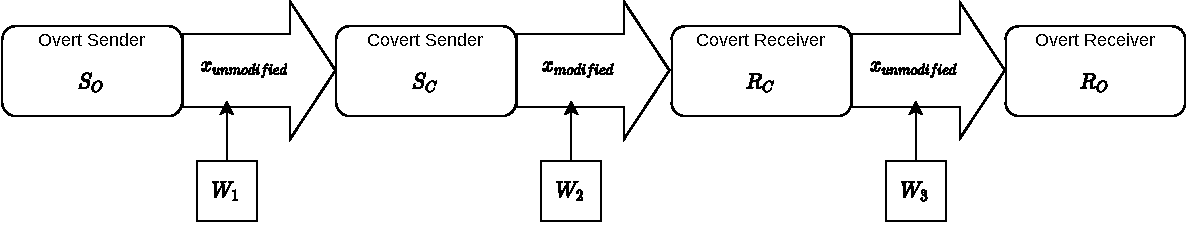
\includegraphics[width=\linewidth]{"figures/reversible_cc.pdf"}
				\caption{Layout of a reversible network covert channel and possible warden placements}
				\label{revcov}
			\end{figure}
			The defining quality of the analysed covert channel is its reversibility. The concept of reversible data hiding originated in image steganography, where it refers to steganographic methods that preserve the possibility of restoring an original image from the altered version into which data has been embedded  \cite{Celik2006}. Similarly, a reversible covert channel is a passive covert channel in which the covert receiver $R_C$ restores the original network packet $x_{unmodified}$ from the incoming covert packet $x_{modified}$ before forwarding it to the overt receiver $R_O$  \cite{Wendzel2015} (c.f. figure \ref{revcov}). \\
			When applicable, reversible covert channels can lead to serious security threats, as they exhibit the relatively noise-free communication of storage channels without sending provably modified traffic to the overt receiver. Their detection is particularly difficult as warden devices placed in between $S_O$ and $S_C$ ($W_1$ in figure \ref{revcov}) and $R_C$ and $R_O$ ($W_3$ in figure \ref{revcov}) will not be able to distinguish traffic belonging to the covert channel from regular network traffic by only observing packet content and ordering. Only wardens on the connection between $S_C$ to $R_C$ ($W_2$ in figure \ref{revcov}) might raise alarm due to altered packet features. However it is entirely possible that this interior connection is outside the observable network of the network operator responsible for the enforcement of the relevant security model $M$. Exterior wardens may only detect the covert channel due to its effects on network characteristics. The easiest measurable network characteristic is latency which is also the only characteristic that can be assumed to be changed by every reversible covert channel in all network environments. Thus latency measurements from $W_3$ might be able to indicate the presence of a reversible covert channel. 
			
			\subsection{Covert Channels Using Hash-Chain-Based One-Time Passwords in TCP}
			%TODO Better Intro
			Keller and Wendzel  \cite{Keller2021} delineated such a computationally intensive reversible covert channel using TCP SYN Hashes. The SYN authentication uses one-time passwords (OTP) as described in  \cite{Lamport} to protect against tampering. \\
			%
			Given a secret key $x$ and a hash function $h$ the series $\{x_i\}$ is defined through the recursive relation 
			\begin{equation}
				x_i = h(x_{i-1})
			\end{equation} 
			with $x_0 = x$.\\
			%
			In order to establish an OTP protected communication the overt sender $S_O$ chooses an arbitrary $n$ and calculates a hash-chain $X = \{ x_0, x_1, ..., x_n\}$. Afterwards $S_O$ shares $x_n$ with authenticator $R_O$ over a secure channel. All following messages can be sent over less secure connections. The $i$-th identification message which $S_O$ sends to $R_O$ will contain the hash $x_{n-i}$. To authenticate the identity of $S_O$, $R_O$ tests if the received hash $x_{rec}$ satisfies \begin{equation}
				h(x_{rec}) = x_{n-i+1}.
			\end{equation} 
			
			By the definition of $\{x_i\}$ this implies that $x_{rec} = x_{n-i}$. Because hash functions are easy to compute but difficult to reverse, this suffices to prove with reasonable certainty that $S_O$ possesses knowledge of the secret password $x$.\\
			The covert channel described by Keller and Wendzel abuses the fact that the upper part of the hash-chain $X$ is shared openly. A symbol $s$ is translated into a number $m = L(s)$ according to a pre-shared alphabet $L$. In order to send this symbol as covert message, the covert sender $S_C$ interrupts a message sent by $S_O$ and flips the $m$-th bit of the hash $x_{n-i}$:
			\begin{equation}
				x_{cov} = flip_m(x_{n-i}).
			\end{equation}
			 The new TCP packet containing the new hash $x_{cov}$ is forwarded to $R_C$, who has knowledge of the last sent hash $x_{n-i+1}$. They consecutively flip each bit of $x_{cov}$ until they find an $m'$ for which 
			 \begin{equation}
			 	h({flip}_{m'}(x_{cov})) = x_{n-i+1}.
			 	\label{cc-equ}
			 \end{equation}
			 To restore the original message $R_C$ replaces $x_{cov}$ with $x_{n-i} = {flip}_{m'}(x_{cov})$. The restored message is forwarded to $R_O$. Because bit-flipping is a self-inverse operation and hash functions are made to be collision resistant, $R_C$ can be fairly certain that $m' = m$. He can now lookup $s = L^{-1}(m)$ inside the pre-shared alphabet. \\
			As hash calculations are generally computationally expensive, this covert channel should create a noticeable increase in network latency. Possible statistical detection mechanisms have been investigated by Schmidbauer and Wendzel \cite{Schmidbauer2021}. They have found mixed success utilizing statistical mean-threshold tests. While covert channels using very computationally intensive sha3 hashes and unoptimized alphabets were relatively easy to detect, recognizing modified network traffic using the faster sha2 or md5 hashes with optimized alphabets proved impossible by threshold detection in many cases. \\
			Besides its reversibility this type of covert channel also offers a relatively inconspicuous non-operational state that can be integrated seamlessly into normal operation to decrease its effect on overall network load. By forwarding the packet without modifying the TCP hash $S_C$ can easily send a packet that will be ignored by $R_C$ after a singular hash calculation  \cite{Schmidbauer}. If $S_C$ only modifies half the packets sent to $R_O$ it can half its effect on network delay. \\
			Another possibility to reduce the generated delay is to reduce the length of the alphabet. By encoding binary digits instead of ASCII symbols into the TCP hash the maximal number of hash calculations can be reduced to three ($flip_0(x_{cov})$ to check whether covert channel is active, $flip_1(x_{cov})$ if $s=0$ and $flip_2(x_{cov})$ if $s=1$). This would of course come at the drawback of significantly reduced covert channel throughput. \\
			By changing the ordering of letters in the alphabet we can also change the effect of the covert channel on runtime. While this procedure can only increase latency compared to the optimal alphabet, the covert channel operator may do this intentionally to hide the channel's effect of on the packet runtime distribution shape when he suspects that shape-aware detection methods are employed. Another possibility to evade detection is to use intentional traffic normalization.
			
			\label{cc-desc}
			
			
		\section{Problem Analysis}
		
			In order to assess the potential success of different detection approaches we describe a basic model of network traffic delay distributions as outlined in the general literature. Afterwards we model the delay specific to the analysed covert channel. We combine these models to develop a mathematical formulation of the problem of reversible covert channel detection. 
		
			\subsection{Statistical Properties of Network Latency}
			
			The following processes contribute to the amount of time $D$ it takes for a given packet to be forwarded from one node $A$ of a network to another node $B$  \cite{Goonatilake2012, Bovy}:
			\begin{itemize}
				\item \textit{Propagation} $D_{pg}$: The time it takes to forward packets from node $A$ to node $B$ at the speed of light within optical fibre (200 $\frac{km}{ms}$  \cite{Cottrel2015}).  
				\item \textit{Transmission} $D_{t}$: Delay caused by the transmission medium. This is mainly related to the actual transmission and reception of the network packet. It is mainly influenced by the size of the packet, choice of physical encoding and characteristics of the transmission medium (Ethernet, wireless, etc.) 
				\item \textit{Queuing} $D_{q}$: Idling of packets when the router / processor cannot process the packet because it is preoccupied with the processing of other packets. 
				\item \textit{Processing} $D_{ps}$: Delay caused by the creation, manipulation and handling of packets. Router Processing (e. g. routing table lookup, IP option handling, header field editing) is difficult to predict, as it is highly dependant of the used protocol and its hardware implementation by the router manufacturer  \cite{Popescu2008}. Sender and receiver processing also exhibit a high dependence on the used protocol as well as the application issuing the network calls. However their effect can be limited by choosing a measurement point outside the sender or receiver operating system.
			\end{itemize}

			These components can be categorized into deterministic and stochastic delay sources  \cite{Bovy}. \\
			Propagation and Transmission are of the deterministic type and can be assumed to stay constant between two packets $p_1$ and $p_2$ if they travel along the same Route $R$ and environmental conditions (e.g. wireless signal quality) remain constant. As the complexity of internet topology increases at larger scales, deterministic delay scales exponentially with physical distance between hosts  \cite{Hillmann2015}. Queuing is generally stochastic, as the amount of packets that are handled simultaneously by any given router varies randomly. Processing contributes in a rather complex way to both stochastic and deterministic delay. \\ 
			Network end-to-end delay has been shown to exhibit seasonality  \cite{Hooghiemstra} due to varying global network load. Additionally random changes in network carrying capacity, the local network configuration and route switching can have an effect on both the deterministic as well as the stochastic elements of $D$  \cite{Bovy}. These effects must be taken into account when analysing measurements of network traffic taken over prolonged periods of time, but can be assumed to be minimal from one packet to the next. \\
			
			It is well known that internet traffic delay exhibits self-similarity  \cite{Crovella1997} and long range dependence  \cite{Kocisky2008}. Self-similarity is the property of fractal data to possess the same correlational structure at different scales. Long range dependence is a closely related phenomenon that describes the persistence of correlation over a wide range of time scales. \\
			This behaviour can be almost entirely traced back to effects influencing the queuing delay  \cite{Willinger1997}. Both the overall queuing delay $D_q$  \cite{Bovy} as well as the individual queue delays $d_q(r)$ at each router $r \in R$  \cite{Popescu2008} are heavy-tailed variables under the following definition from  \citeauthor{Cooke2011}  \cite{Cooke2011}: 
			\begin{definition}[heavy-tailed variables]
				Let $F(x)$ denote the distribution function of a random variable $X$. We shall call $X$ heavy tailed if its survival function $S(x) = 1 - F(x)$ has a polynomial decay rate, i. e.: 
				\begin{equation} \frac{S(x)}{x^{-\alpha}} = O(1)\text{ as } x \rightarrow \infty
				\end{equation}
				for some tail index $\alpha \in \mathbb{R}^+$
			\end{definition}
			It can be shown that for all $\kappa \in \mathbb{N}$ with $\kappa \geq \alpha$ the $\kappa$-th moment of $X$ is infinite  \cite{Cooke2011}. Willinger et al.  \cite{Willinger1997} showed that $1 < \alpha < 2$ can be assumed for the distribution of $d_q(r)$. It follows that $Var(d_q(r)) = \infty$, which means that the central limit theorem does not apply. They further demonstrated that the heavy-tailedness and self-similarity of  $D_q = \sum_{r \in R} d_q(r)$ arises from the heavy-tailedness and infinite variance of its individual components $d_q(r)$.\\
			This result agrees with experimentally determined distributions of $D$ 
			 \cite{Fremond2021, Pfitzinger2018a, Pfitzinger2018, Papagiannaki2003}. However there is no conclusive result on the heavy-tailed distribution that best fits network traffic delay. A Pareto distribution with 
			\begin{equation}
				\label{pareto}
				S(x) = {\left( \frac{x}{x_0} \right) }^{-\alpha} 
				\text{ for } x > x_0
			\end{equation} 
			 can be fit very well to the tail of the overall distribution  \cite{Pfitzinger2018a, Fremond2021}. At its peak the distribution requires a more curved function to correctly model its behaviour. This peak is fairly sharp compared to other heavy-tailed distributions (such as the one of the investigated covert channel). Log-normal and Beta  \cite{Pfitzinger2018a} as well as Weibull  \cite{Papagiannaki2003} distributions have been fit to network traffic delay with high degrees of success.\\
				%
			The feature extraction process of both machine learning approaches developed as part of this thesis discards information about the chronological sequence of latency measurements. Because $D$ exhibits long-range dependence this cannot be done trivially. However compared to actual time-series data streams, this long-range dependence appears functionally only as another kind of random noise. In chapter 3 and 4 we use the assumption that $D$ can be modelled as random variable and is thus temporally symmetric while choosing statistical measures and generating larger training datasets by random sampling.
			\label{network-lat}
			
			%%
			%TODO Image deterministic vs stochastic delay
			%%
			%TODO possibilities of analysing it as a time series
			
			\subsection{Covert Channel Delay Modelling}
			
			Let $\gamma$ be the delay caused by the analysed covert channel. The covert channel operation can be split into a deterministic and a stochastic component. We will denote the former with $\gamma_0$. It is comprised of the processing time necessary to capture the packet message $M$, perform the lookup in the shared Alphabet $L$ and set up the hash loop. The stochastic delay consists of the necessary time to calculate the hash $h(flip_i(M))$ until $i=L(s)$. Let $\hat{h}$ denote the time necessary to perform this operation. We can now express the delay necessary to send the symbol $s$ over the covert channel as:
			\begin{equation}
				\gamma(s) = \gamma_0 + \sum_{i=1}^{L(s)}{\hat{h}(flip_i(M))}.
			\end{equation}
			Because hash functions are designed to reduce computation time dependence on input size and content, the assumptions that $\hat{h}(x) \approx H$ for some constant $H$ and $y_0 \approx 0$ can be made to simplify this formula to:
			\begin{equation}
				\gamma(s) = H L(s).
			\end{equation} 
			The form of the probability distribution of $\gamma$ is thus dependant on the message $\{s_i\}$ being transmitted and the alphabet $L$ that is used. It is further scaled by the parameter $H$ which is influenced by the choice of hash algorithm and the hardware on which it is performed.\\
			For natural text using the optimal alphabet $L_0$ we can expect $\gamma$ to follow Zipf's law  \cite{zipf_web, Corral2015}. It states that the frequency of the letter of rank $r$ equals \begin{equation}
				p_r = \frac{r^{-\alpha}} {\sum_{n=1}^{N}{n^{-\alpha}}}
			\end{equation}
			where $\alpha$ is a tail index dependant on the specific data and $N$ is the number of elements  \cite{zipf_web2}. The Zipf distribution is essentially a truncated discrete version of a Pareto distribution, as will be demonstrated in the following chapter (c.f. figure \ref{cc-fig}).\\
			For compressed or encoded data a more uniform profile can be expected. For unoptimized alphabets or normalized covert traffic flow we can expect $\gamma$ to possess a less distinct, more dense distribution with a lighter tail.\\
			In general we may use the following formulation of this thesis' problem statement:
			\begin{definition}[Problem Statement]
				Given a warden positioned at $W_3$ in between a potential covert receiver $R_C$ and the overt receiver $R_O$, it is impossible for this warden to detect a reversible covert channel by analysing the packet stream ordering or the packets themselves. We assume that the covert channel leaves traces of its existence only in the form of network delay. The warden can observe the network delay as a stream of inter packet times $D^*$. It is now tasked with deciding whether $D^*$ displays qualities that resemble those of unmodified traffic $D$ or if it is being modified by a computationally intensive covert channel, causing it to resemble $D + \gamma$ instead.
			\end{definition}
			
		
		\section{Data Stream Classification}
		
			Low dimensional Data streams pose a unique challenge for traditional classification models, especially machine learning algorithms\cite{Faouzi2022}: Most models take ordered data vectors of fixed length as input and rely generally upon the fact that the relationship between components of this vector and the result is similar across different observations. For data streams, there is no intuitive natural length or starting point for this input vector and its components are mostly interchangeable. This makes directly inputting data streams into classification or regression algorithms a bad idea. Most literature we found about low dimensional data streams dealt with time series data (measurements taken at fixed intervals). Here it is explicitly assumed that a strong correlation between neighbouring values exists. However, in the classification of random variables like $D^*$ this is not the case, as values of $D^*$ are only weakly correlated through long range dependence.\\
			Additionally data streams face the problem of concept drift, which occurs when the properties of a data stream change gradually during data collection  \cite{Janardan2017}. Concept drift can occur within classes as well as across classes. The network delay $D^*$ might for instance change its distribution because of the presence of a covert channel, it might however also change due to increased global network load.\\
			For an algorithm that should be trained in real time, data stream classification also faces various performance and timing constraints that need to be addressed when designing the algorithm. While this thesis will not addresses these issues, a comprehensive overview of various approaches for real-time training in data stream classification can be found in  \cite{Nguyen2015}. \\
			
			In order to offset the disadvantages faced when dealing with data streams most machine learning approaches heavily preprocess and feature engineer data streams before applying actual machine learning algorithms  \cite{Faouzi2022}. Time series classification usually involves scaling and modifying the data in order to classify it based on its general shape (cf. Shapelet-based algorithms, Dynamic Time Warping). This process can be supported by selecting windows of fixed or random length from the data stream and computing statistical measures (cf. Proximity Forest, Bag-of-Words).\\
			Tree based algorithms using statistical measures of subsets are well suited to the task of data stream classification as many problems are well suited to be solved by a series of binary decisions. Neural networks are also heavily used due to their ability to quickly and accurately reproduce non-linear processes  \cite{Faouzi2022, Zhao2021}.\\
			Alternatively the data can be transformed into a one or more dimensional representation of itself. Examples include Fourier transforms, recurrence plots, angular fields, Markov transition fields  \cite{Faouzi2022} and empirical probability distributions / histograms  \cite{Zdravevski2015, Plaud2019}. These representations may be more susceptible to analysis with machine learning techniques and can make use of more sophisticated algorithms found in the domain of image recognition due to the inherent structure of these representations. Additionally they enable an approach of analysis that can ignore or highlight certain aspect of the data such as their temporal layout. \\
			Convolutional kernels ar one such technology from the domain of image recognition that may be applied either directly to the data itself or to various representations of it. Convolutional kernels are convolved with the input data via a sliding dot product and serve to capture abstract representations of regions, shapes and geometrical features contained within the data. They have been exceptionally successful in the classification of images as well as time series. Because they are linear operations they can be seamlessly integrated into neural networks to create convolutional neural networks or randomly generated to access greater feature variety, as demonstrated in  \cite{Dempster2020}.\\
		
			Data stream classification has been applied with great success to internet packet data with applications mainly in network management and security.  \cite{Zhao2021}, \cite{Pacheco2019} and  \cite{Shahraki2022} offer an overview of state of the art approaches and solutions. Included in  \cite{Zhao2021} is a list of publicly available datasets and a comparison of commonly used machine learning algorithms. Most classifiers use general statistical measures and packet contents for classification. Although statistical fingerprinting alone has been shown to be sufficient for traffic classification in some situations  \cite{Crotti2007}.\\
			Network orchestrators may use traffic classification for efficient load balancing and packet prioritization  \cite{Manjunath2021}. Its application has also been tested in the context of internet of things  \cite{Pathmaperuma2022}.  \cite{Chourib2019} and  \cite{Saeli2020} used machine learning models to detect covert channels in IP traffic streams.  \cite{Epishkina2019a} outlined the usage of machine learning algorithms to improve the detection of inter-arrival time covert channels.  \cite{Velasco-Mata2021} detected botnet traffic via machine learning classification of network traffic. \\ 
			 \cite{Williams2006} compared the performance of five Bayesian and Decision Tree algorithms. Graph networks  \cite{Pang2021} and convolutional neural networks  \cite{Wang2018} also showed success in classifying network traffic. \cite{Al-Eidi2021} transformed inter arrival times into 2 dimensional pixel arrays in order to take advantage of sophisticated convolutional neural network image recognition algorithms to detect covert timing channels.
			
			
	%---------------------------------------------------------
	%						Exploration
	%---------------------------------------------------------
	\chapter{Detection Approaches}
		
		We will outline possible solutions to the problem of detecting unnatural network delay caused by a computationally intensive covert channel. First we delineate on the origin of the network traffic data we used. Afterwards statistical features of the collected data are explored and assessed towards the possibility of efficient detectability. Based on this various approaches for covert channel detection are described. These include simple threshold tests for the various statistical properties, machine learning algorithms for the classification of these statistical measures and convolutional neural networks that operate directly on a histogram representation of the data. 
		
		\section{Data Acquisition}
			
			Schmidbauer and Wendzel  \cite{Schmidbauer2021, Schmidbauer} implemented the discussed covert channel into a physical system and performed inter packet measurements. Their system consisted of four interconnected raspberry Pi that would serve as $S_O$, $S_C$, $R_C$ and $R_O$. They made measurements on this system available to us. This data has the clear advantage that it is collected from a physical implementation of the covert channel and doesn't suffer from simulation error. However because of the design of their setup, the measurements possess significant (albeit constant) network delay. This reduces the applicability of their data to a broader spectrum of situations and minimizes the impact of the covert channel relative to the traffic delay. The comparatively small size and variability of their dataset also proved disadvantageous for statistical analysis and machine learning. \\
			\begin{table}
				\begin{tabular}{|m{4cm}|m{9cm}|m{2cm}|}
					\hline
					Dataset & Description & Used In \\
					\hline
					\hline
					Physical measurements &
					Measurements taken from physical implementations of hash-chain covert channel provided by Schmidbauer and Wendzel  \cite{Schmidbauer} &
					Figure \ref{Schm-perf}\\
					\hline
					Self-measured data &
					Self-made ping measurements from a home computer with simulated covert channel runtimes added after data production&
					Sections \ref{assessment}, 3.3 and 4.2\\ 
					\hline
					RIPE Atlas data&
					RIPE Atlas data \cite{RIPE} collected from the 20th of April 2022, filtered to only include heavily pinged connections ( > 100 pings available) with simulated covert channel runtimes added after data production &
					Section 3.3\\
					\hline
				\end{tabular}
				\caption{Datasets used as part of this thesis}
				\label{dataset-tab}
			\end{table}
			In order to better study an optimised implementation of the covert channel described in chapter \ref{cc-desc} on multiple connections as well as to significantly increase the amount of data available, we have decided to simulate the delay caused by the covert channel and add them to legitimate but unrelated network traffic data in order to simulate covert traffic.  We have sourced this data from the RIPE Atlas database of network measurements as well as from self-captured ping measurements. All datasets that were part of this thesis as well as their place of usage can be found in table \ref{dataset-tab}; the structures of the datasets can be observed in figures \ref{mean-fig} and \ref{peak-width-fig} later in this chapter.\\
			Self-measured ping data was collected using scapy \cite{scapy} from a private laptop within a private network. The measurements were taken in measurement sessions of 1000 or 4000 pings to a number of different IP addresses. In order to increase the available data depth for machine learning training we decided to perform between 15 and 30 measurement sessions for the six connections listed in table \ref{connections-tab} over an average time period of one day. We choose very short connections within the local network over Ethernet and WiFi, the Google DNS server as a low latency connection outside the local network, two popular websites (euronews.com and ebay.com) as medium latency connections and the DNS server of an Australian ISP (Telstra) as high latency connection. 
			\pagebreak\\
			Additionally we stripped data from the RIPE Atlas database of network measurements \cite{RIPE}. RIPE Atlas uses specialised devices that ping each other and many public-facing IP addresses on a daily or hourly basis. We downloaded the publicly available dataset of all RIPE ping measurements made on the 20th of April and searched for source -- destination address pairs that occurred more than 100 times within the ping measurements. In total we have collected 1195 connections with an average number of 2020 pings per connection. We chose this method to increase the repeatability of our observations from section 3.3 and guarantee a sufficient width for the observed dataset. \\
			
			\label{script}
			In order to simulate the effect of a physical covert channel using TCP hashes on network delays, we wrote a script that measures the delay produced by the covert channel described in section \ref{cc-desc}. We assumed that capture and forwarding of packets can be done in negligible time. Given an alphabet $L$, a hash function $h$ and a text written in natural language we defined the routine in figure \ref{cov.sim} to simulate the covert channel delay.\\
			\begin{figure}[t]
				\rule{\linewidth}{0.4pt}
				\begin{algorithmic}[1]
					\State $\text{c = random.choose(text)}$
					\State $\text{start = now();}$
					\For {$ \text{a }in \text{ } L$}
					\State $h\text{(text + c);}$
					\If {$\text{a} == \text{c}$}
					\State $break$
					\EndIf
					\EndFor
					\State \Return $\text{now() - start;}$
				\end{algorithmic}
				\rule{\linewidth}{0.4pt}
				\caption{Algorithm used to simulate covert channel runtimes}
				\label{cov.sim}
			\end{figure}
			In our measurements we have always taken $L$ to be the optimal ASCII alphabet for the given text, an excerpt from "Alice in Wonderland". We used the md5, sha256, sha3\_256,
			sha384 and sha3\_512 hash functions as implemented in the python hashlib package. Figure \ref{cc-fig} shows the empirical probability distribution of the simulated $\gamma$ for these hash functions. All of them clearly show a discrete, heavy-tailed Zipf-distribution convoluted with the runtime distribution of the various hash functions. The hash algorithm with the longest runtime sha3-512 (d) displays this pattern the strongest, while for the short sha256 (a) and md5 (e) algorithms the individual peaks almost merge into one continuos Pareto-like distribution.
			
			\begin{table}
				\begin{tabular}{|m{3cm}|m{6cm}|m{2.5cm}|m{3cm}|}
					\hline
					Connection name / IP Address & Target & Connection Type & Latency Range[$ms$] \\
					\hline
					\hline
					lan & home server within local network & Ethernet & 1-20 \\
					\hline
					wlan & home server within local network & Wireless & 15-20 \\
					\hline
					8.8.8.8 & Google DNS server& Wireless & 10 - 15 \\
					\hline
					81.92.228.153 & euronews.com & Wireless & 15-30 \\
					\hline
					66.211.175.229 & ebay.com & Wireless & 150-250 \\
					\hline
					139.130.4.5 & Telstra DNS Server & Wireless & 300-350 \\
					
					\hline
				\end{tabular}
				\caption{Main Targets of self-made ping measurements}
				\label{connections-tab}
			\end{table}
			
		\begin{figure}
			
			\begin{subfigure}{0.5\textwidth}
				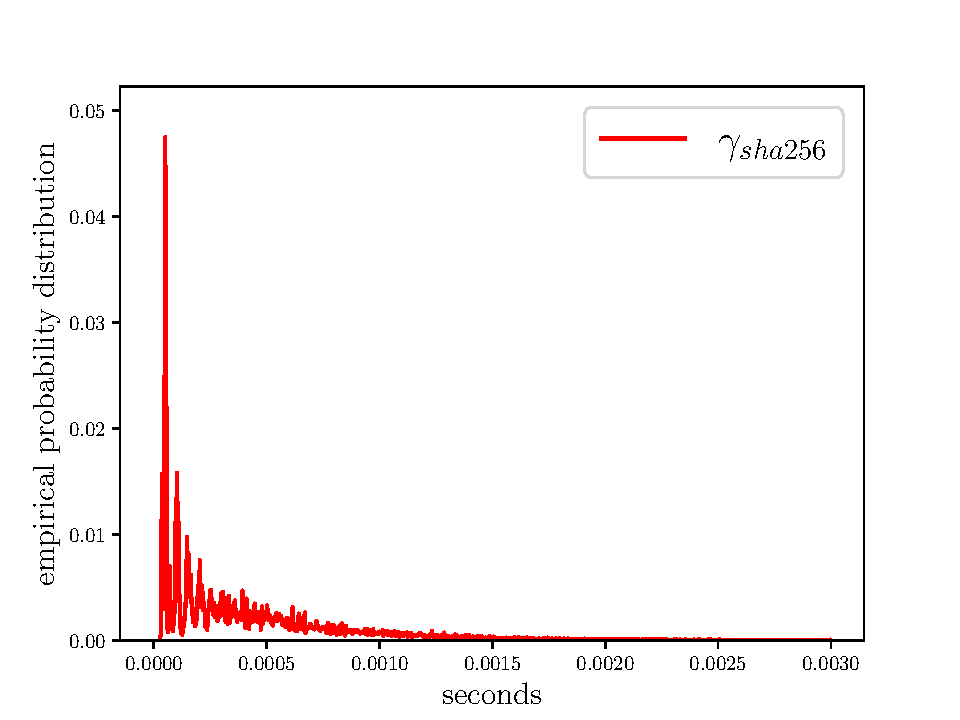
\includegraphics[width=0.98\textwidth]{figures/_CC_compare_completeopenssl_sha256_cc_3_light.pdf}
				\caption{sha256}
			\end{subfigure}
			\begin{subfigure}{0.5\textwidth}
				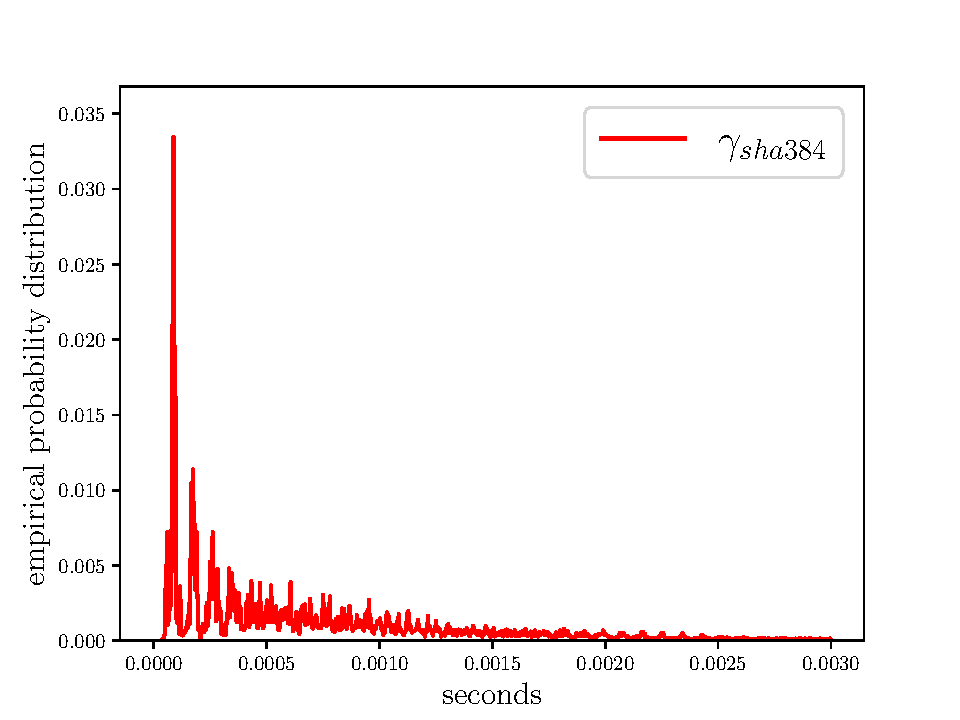
\includegraphics[width=0.98\textwidth]{figures/_CC_compare_completeopenssl_sha384_cc_0_light.pdf}
				\caption{sha384}
			\end{subfigure}
			\begin{subfigure}{0.5\textwidth}
				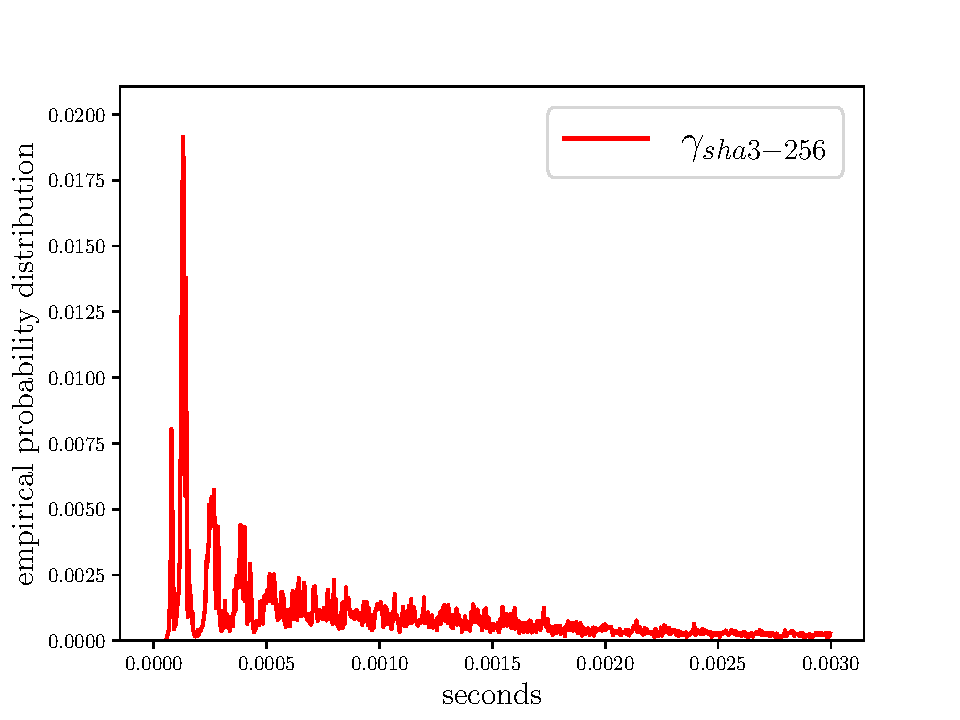
\includegraphics[width=0.98\textwidth]{figures/_CC_compare_completeopenssl_sha3_256_cc_0_light.pdf}
				\caption{sha3-256}
			\end{subfigure}
			\begin{subfigure}{0.5\textwidth}
				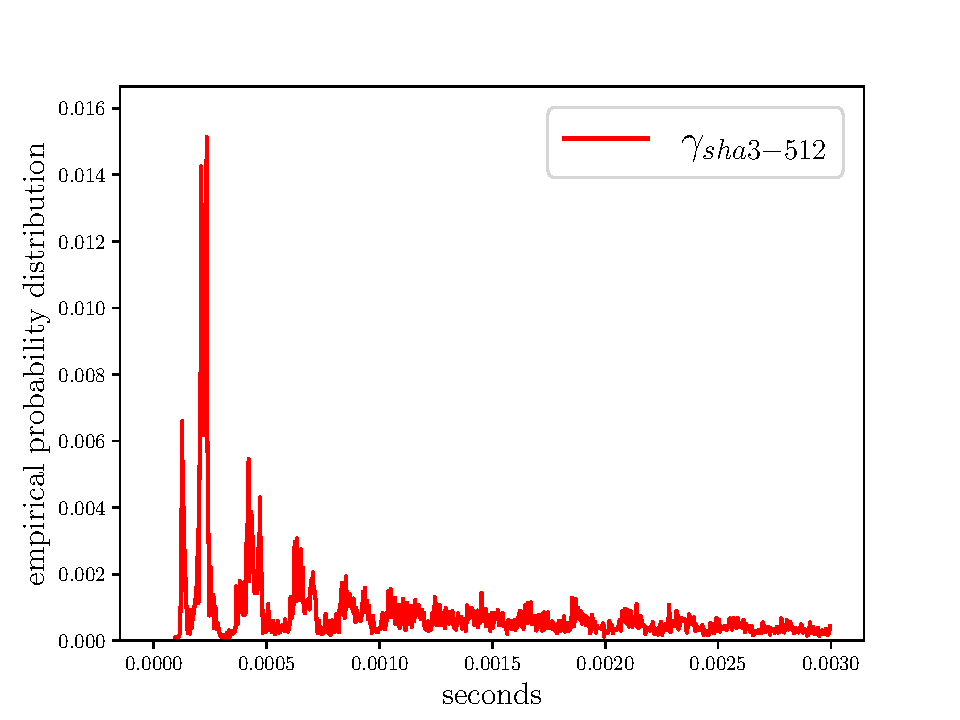
\includegraphics[width=0.98\textwidth]{figures/_CC_compare_completeopenssl_sha3_512_cc_0_light.pdf}
				\caption{sha3-512}
			\end{subfigure}
		
			\centering
			\begin{subfigure}{0.5\textwidth}
				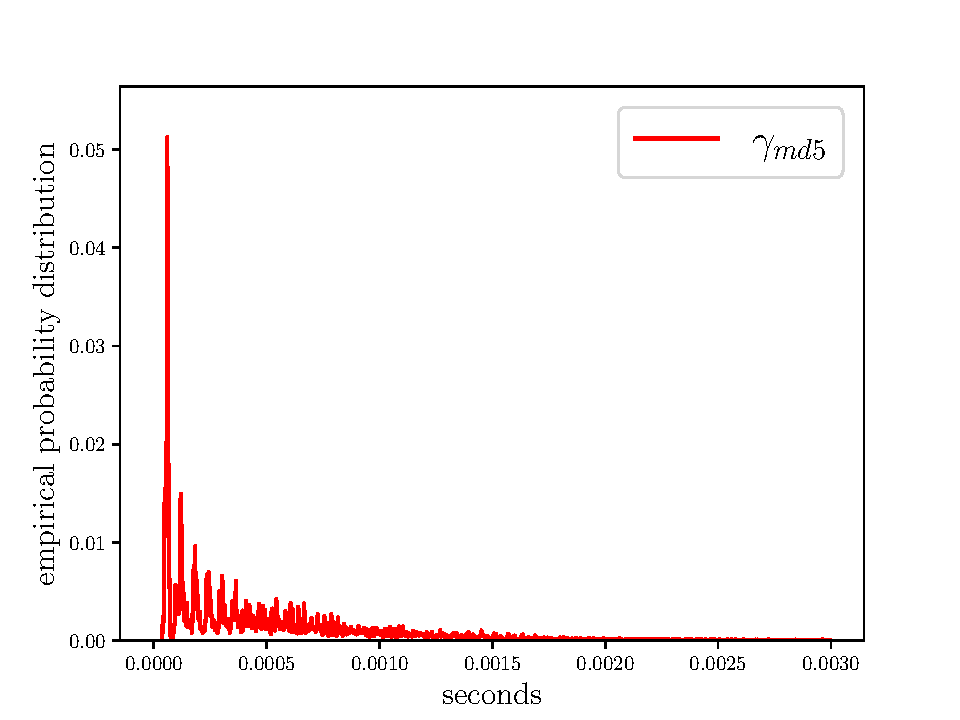
\includegraphics[width=0.98\textwidth]{figures/_CC_compare_completeopenssl_md5_cc_0_light.pdf}
				\caption{md5}
			\end{subfigure}
			
			
			\caption{Simulated covert channel empirical probability distributions}
			\label{cc-fig}
		\end{figure}
			
		%%%%%%%%%%%%%%%%%%%%%%%%%%%%%%
		%  Data Exploration
		%%%%%%%%%%%%%%%%%%%%%%%%%%%%%%
			
		
		\section{Assessment of Detectability}	
			
			\label{assessment}
			\label{assessment2}
			We try to determine qualitatively significant differences between natural and modified network traffic and determine whether a detection of the covert channel is possible against the backdrop of the natural variability of network traffic delay. Broadly speaking there are three different passive design approaches for a an exterior warden ($W_3$ in figure \ref{cc-fig}) that can detect  a reversible covert channel in traffic $D^*$ from a connection $R$:
			\begin{itemize}
				\item \textbf{Absolute Detection}: A fixed model that, given $D^*$ collected from any $R$, is able to classify it as belonging to $D$ or $D + \gamma$
				\item \textbf{Specific Detection}: A model adjusted to a single $R$ (or a constant set of connections $\{R_0, ..., R_n\}$) that can accurately classify $D^*$ only on that connection
				\item \textbf{Relative Detection}: A flexible model that can classify traffic from any connection $R$, but needs to be adjusted to the specific connection either through parametrization or by collecting training data from $R$
			\end{itemize}
			Absolute detection is the hardest to implement and could be practically impossible if inter connection differences in $D$ can mirror the effects of adding $\gamma$ to $D$. Specific detection is relatively simple to set up and could produce results with very high confidence, but is susceptible to cold start problems and could be confused by natural intra connection differences such as seasonal shifts in network load or a switch from Ethernet to Wi-Fi. Relative detection would, if  correctly implemented, combine the advantages of the other two detection approaches to offset their shortcomings. In chapter 4 we will quantitatively present positive evidence for the efficacy of specific detection approaches and  indication of the potential for the implementation of absolute detection on the set of connections listed in table \ref{connections-tab}. \\
			In general, the following ways of implementing relative detection present themselves:
			\begin{itemize}
				\item The input vector of the machine learning model can be appended with information about $R$ (e.g. hop length, previous average latencies, ...)
				\item Instead of categorising the network traffic the model tries to predict an easily measurable property of the connection (such as hop length). Errors in this prediction can be interpreted as unnatural network behaviour and thus indices of covert channel presence
				\item The classifier consists of multiple machine learning models that are trained for different classification scenarios and switches dynamically between them
				\item The base classifier dynamically learns the properties of the connection during its lifetime 
			\end{itemize}
			In this thesis we focus on sliding window algorithms, e.g. algorithms that take in a fixed number of recent measurements as inputs, however implementations with dynamically shifting window size are also conceivable. Sliding window algorithms allow the relatively easy implementation of detection methods based on statistical models and representations as the input size remains constant and scalability of metrics as well as possible effects of the representation's granularity need not be considered.
			\label{assess_var}
			Figure \ref{comparison-fig} compares the empirical probability distributions of $D$ and $D+\gamma$ for the relatively time-efficient md5 hash function and the very computationally intensive sha3-512 function for data taken from the connections listed in table \ref{connections-tab}. The top graph of each subfigure depicts the histogram of the measurement session with the lowest average ping time and the bottom graph the one with the highest average ping for each connection. \\
			Common to all modified latency data is the increased broadness of its peaks compared to the unmodified data. As is expected, the higher the latency of $D$, the less is differs from $D+\gamma$, with the only noticeable difference between $D$ and $D + \gamma$ in (d) being the lower peak of the histogram, which becomes almost unnoticeable in the higher average latency bottom dataset. When a sharp peak at low latency, such as the one in the top figure of (a) is modified, $D+\gamma$ will noticeable carry over the discrete peaks from \ref{cc-fig}. This effect vanishes however with broader peaks (b) or even slightly higher latency (c). In addition natural traffic at this scale can display similar peaks, such as those seen in the bottom figure of (a). \\
			Comparing the top and bottom figures in \ref{comparison-fig} shows that the impact of random variation on $D$ is generally larger than the effect of the covert channel. This is especially true for connections with very low (a) or very high (f) latencies. For the former because of the significant difference between high and low network or operating system load, for the latter because of the seasonal variability of that type of connection. A comparison of the standard deviation of $D$ to the average size of $\gamma$, as is done in figure \ref{mean-fig}, further enforces this point.
			However the impact of $\gamma$ on the shape of the empirical probability distribution is distinctive enough to be measurable, as most natural distributions, even at high latencies, preserve a sharp peak (c.f. \ref{peak-width-fig}). For distributions where this is not the case, such as the bottom figure of \ref{comparison-fig} (f), only minor changes occur when adding $\gamma$, meaning that a potential covert channel could be truly undetectable.\\
			
			\begin{figure}
				\centering
				\begin{subfigure}{0.32\textwidth}
					\centering
					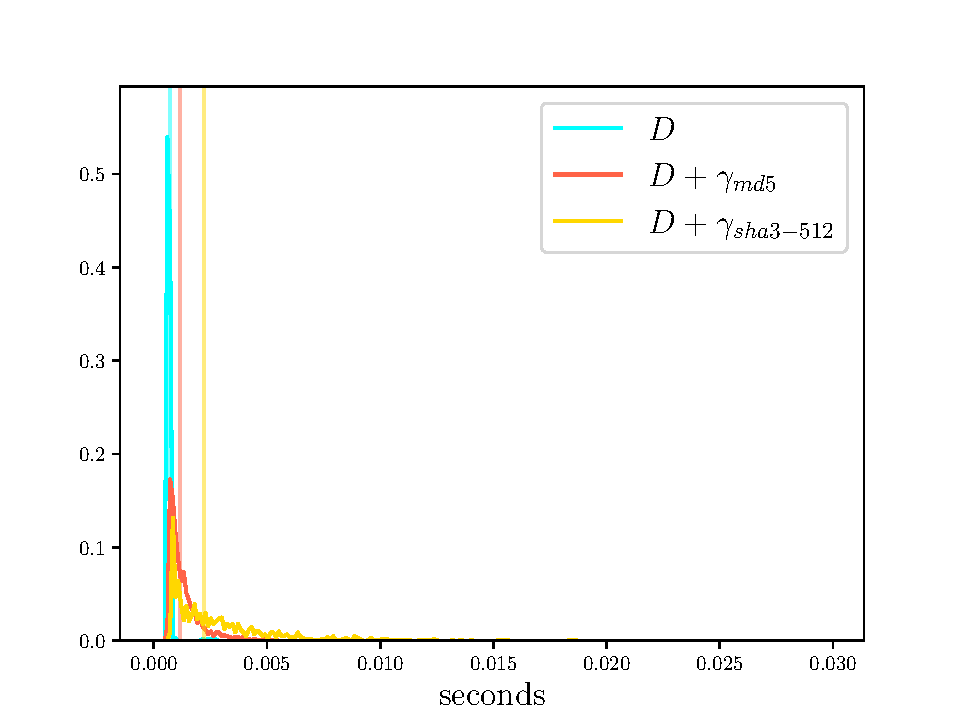
\includegraphics[width=0.98\textwidth]{figures/_LAN_complete_light.pdf}
					\includegraphics[width=0.98\textwidth]{figures/_LAN_complete_dark.pdf}
					\caption{Target within local network\\(via Ethernet)}
				\end{subfigure}
				\centering
				\begin{subfigure}{0.32\textwidth}
					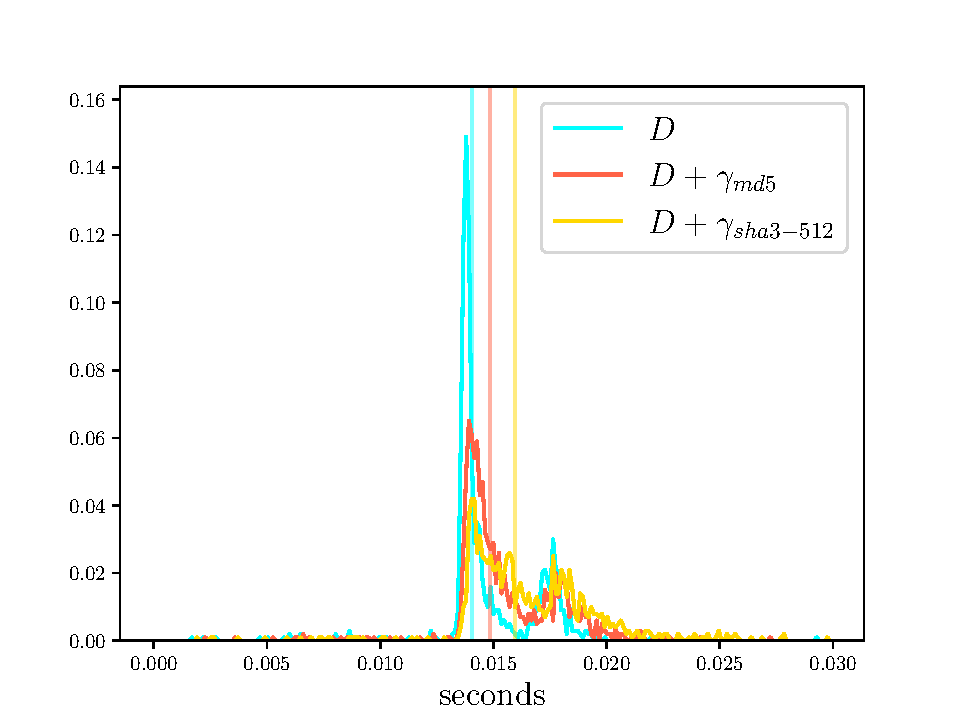
\includegraphics[width=0.98\textwidth]{figures/_WLAN_complete_light.pdf}
					\includegraphics[width=0.98\textwidth]{figures/_WLAN_complete_dark.pdf}
					\caption{Same target \\(via wireless connection)}
				\end{subfigure}
				\centering
				\begin{subfigure}{0.32\textwidth}
					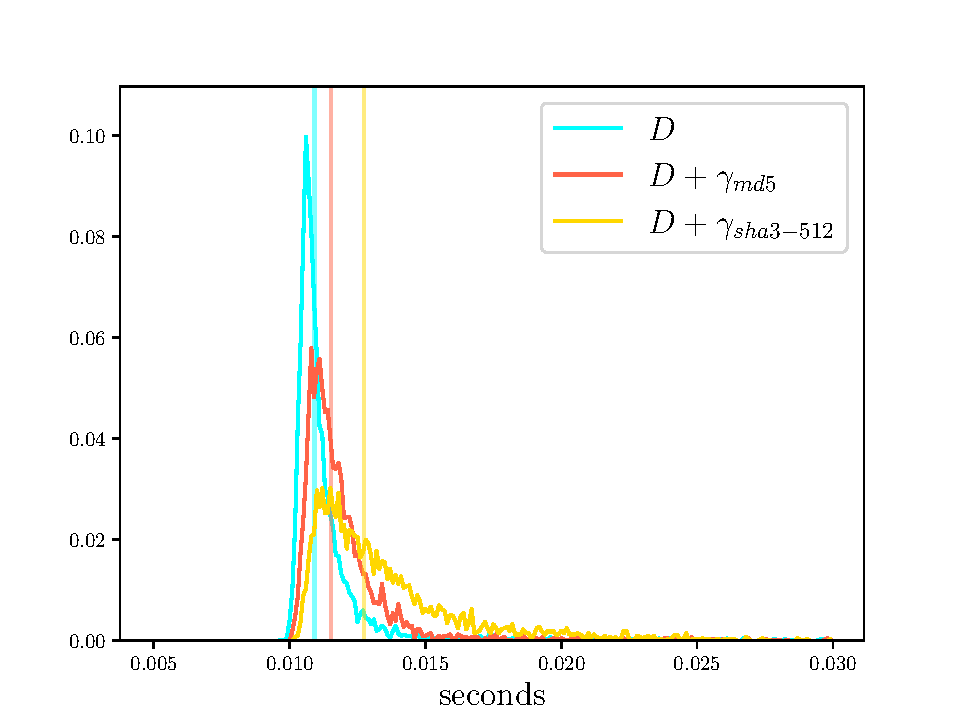
\includegraphics[width=0.98\textwidth]{figures/_GOOGLE_complete_light.pdf}
					\includegraphics[width=0.98\textwidth]{figures/_GOOGLE_complete_dark.pdf}
					\caption{IP 8.8.8.8\\(via wireless connection)}
				\end{subfigure}
				\centering
				\begin{subfigure}{0.32\textwidth}
					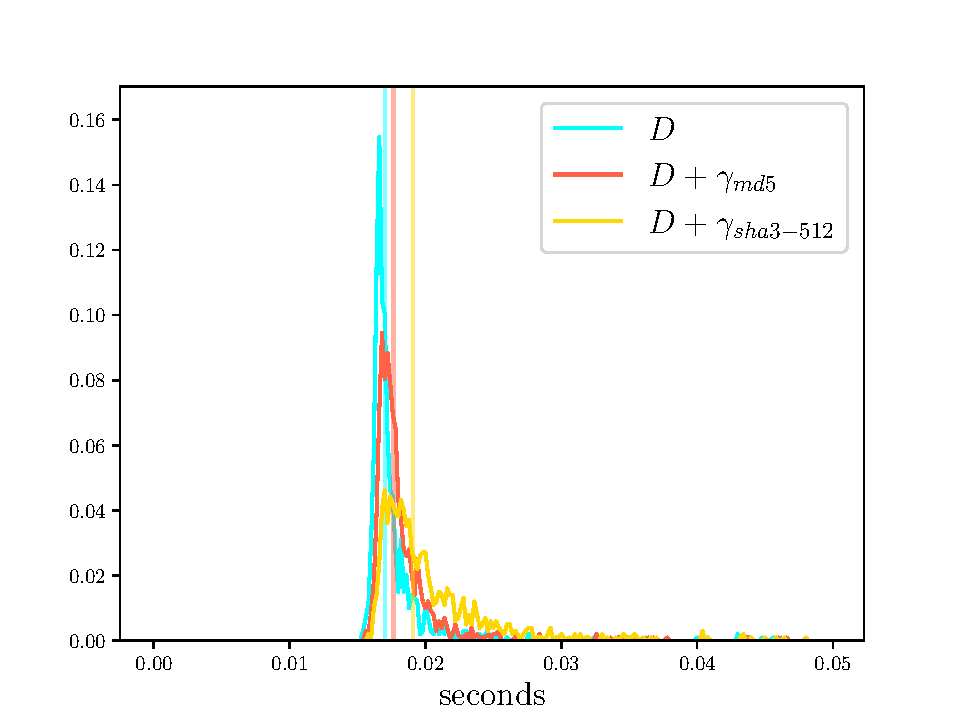
\includegraphics[width=0.98\textwidth]{figures/_MEDIUM2_complete_light.pdf}
					\includegraphics[width=0.98\textwidth]{figures/_MEDIUM2_complete_dark.pdf}
					\caption{IP 81.92.228.153\\(via wireless connection)}
				\end{subfigure}
				\centering
				\begin{subfigure}{0.32\textwidth}
					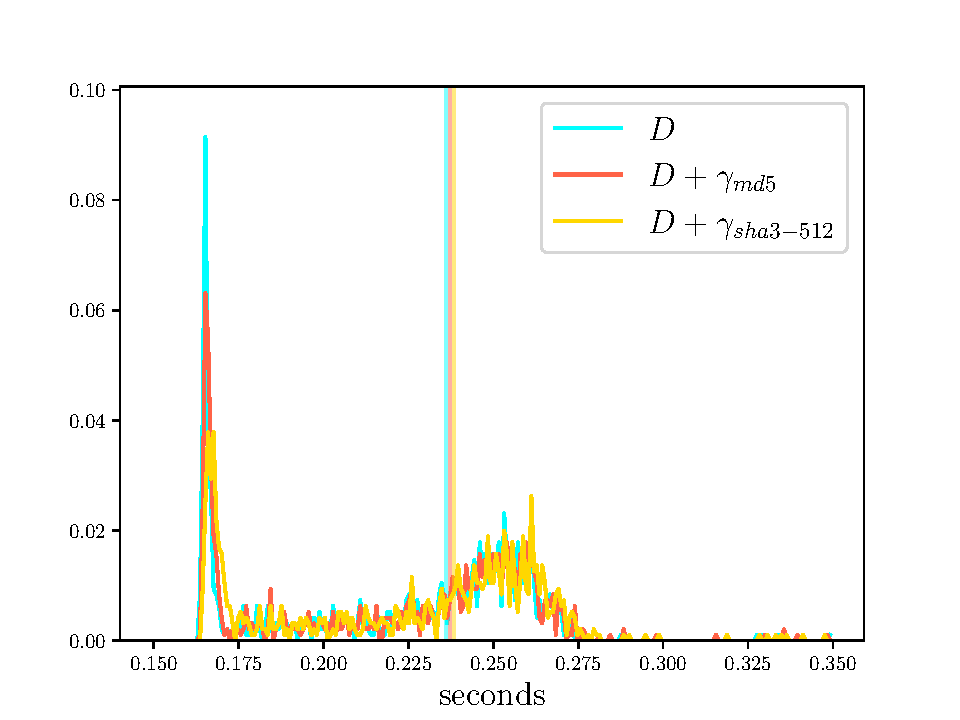
\includegraphics[width=0.98\textwidth]{figures/_MEDIUM_complete_light.pdf}
					\includegraphics[width=0.98\textwidth]{figures/_MEDIUM_complete_dark.pdf}
					\caption{IP 66.211.175.229 \\(via wireless connection)}
				\end{subfigure}
				\centering
				\begin{subfigure}{0.32\textwidth}
					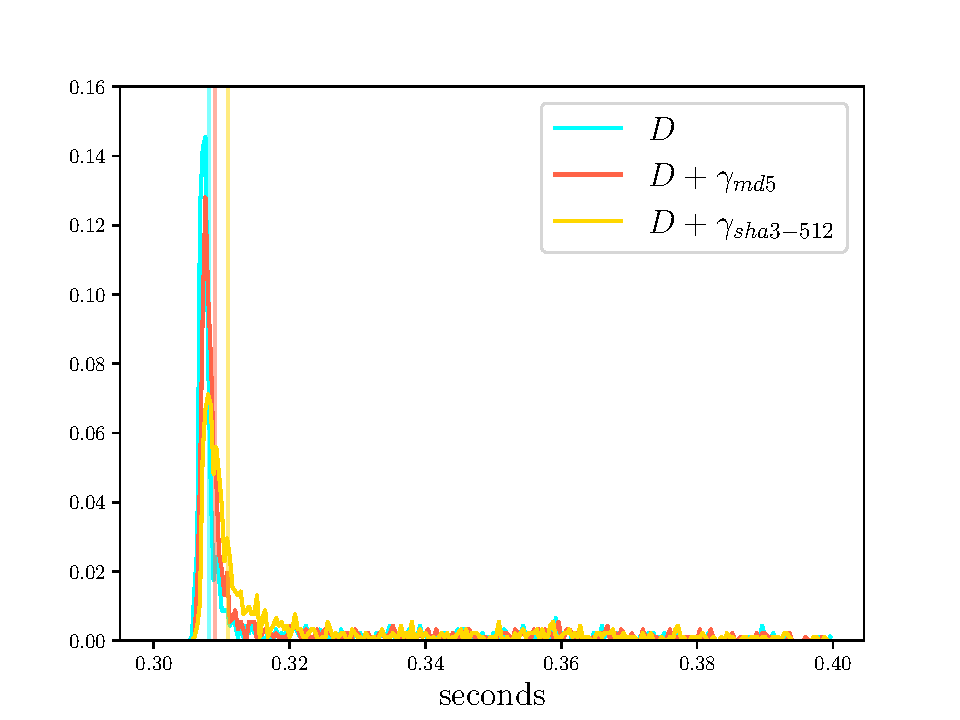
\includegraphics[width=0.98\textwidth]{figures/_AUS_complete_light.pdf}
					\includegraphics[width=0.98\textwidth]{figures/_AUS_complete_dark.pdf}
					\caption{IP 139.130.4.5 \\(via wireless connection)}
				\end{subfigure}
					\begin{subfigure}{0.32\linewidth}
					\hphantom{a}
				\end{subfigure}
				
				\caption{Impact of covert channels using md5 and sha3-512  hashes with the optimal alphabet $L_0$ on the empirical probability distribution of self-made measurements for different connections (c.f. table \ref{connections-tab}). Upper graphs show lowest average latency, lower graphs highest average latency measurement session performed on the connection. The vertical lines indicate the median value of the given empirical probability distribution}
				\label{comparison-fig}
			\end{figure}
			
			\begin{figure}
				\centering
				\begin{subfigure}{0.49\linewidth}
					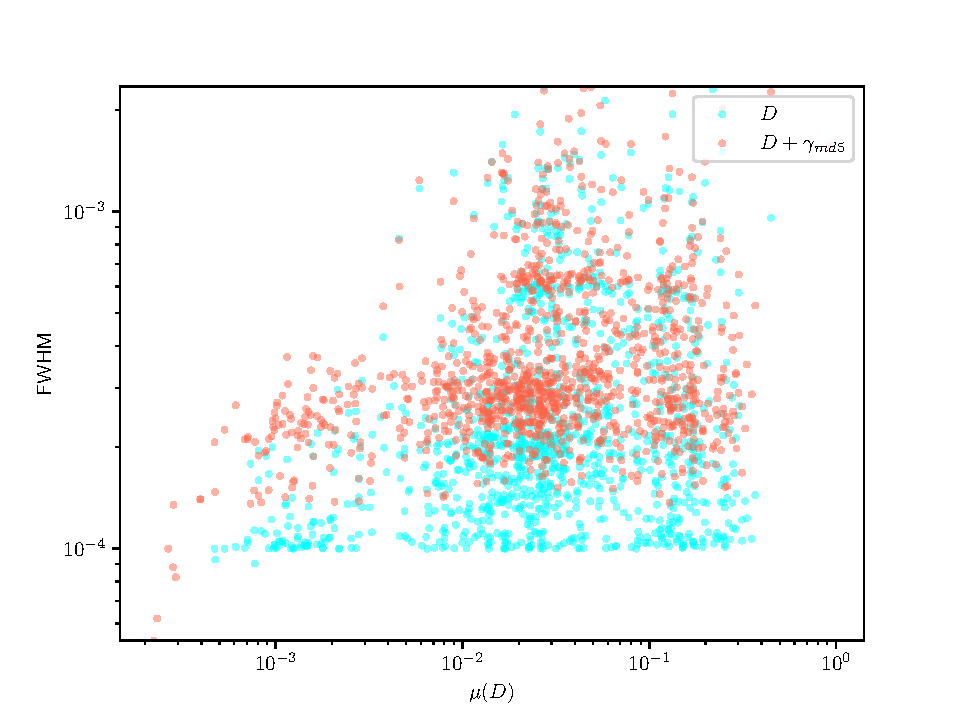
\includegraphics[width=\linewidth]{figures/stat_md5_0FWHM_logscale.pdf}
					\caption{RIPE Atlas dataset}
				\end{subfigure}
				\begin{subfigure}{0.49\linewidth}
					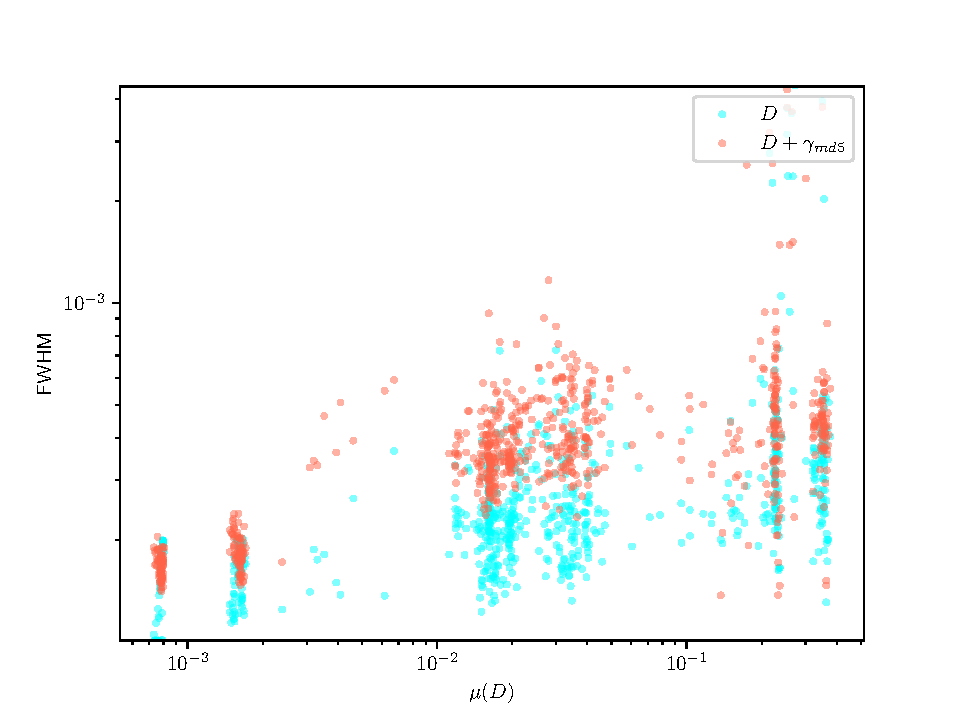
\includegraphics[width=\linewidth]{figures/stat_md5_00all_FWHM_logscale.pdf}
					\caption{Self-made measurements}
				\end{subfigure}
			\caption{Log-log plot of peak width of empirical probability distributions measured as full width at half peak of maximum (FWHM) for $D$ and $D + \gamma_{md5}$}
			\label{peak-width-fig}
			\end{figure}
			
		\section{Statistical Measure Analysis}
		
		\label{measure-list}
		We investigated various statistical measures $\alpha$ for their ability to detect the shape change induced by the addition of $\gamma$ listed in table \ref{measure-tab}. Aside from the  well known measures of mean, median, mode \footnote{calculated as the index of the maximum value of a fine-grained histogram of $D^*$}, standard deviation, skewness and kurtosis, we also investigated several measures of tail heaviness, as the main effect of adding $\gamma$ observed in \ref{comparison-fig} were wider peaks and a heavier tail. \\
		These measures include the Hill \cite{Cooke2011} and Pickands \cite{Pickands1975} tail estimators implemented in the python package developed in the paper \cite{Voitalov2019}. They represent estimations of the exponent from equation 2.6 that use the relationships between the biggest $k$ values of a distribution. This $k$ can be empirically optimized to produce an accurate value for the tail index of many distributions as was shown in the paper.\\
		The Süssmann measure \cite{Sussmann1997} is a relative measure of scale that describes the density of a probability distribution $p$ through the squared height of its probability density function. It is used in quantum mechanics and particle physics as a measure of scale for topologies where a variance cannot be defined straightforwardly. However its discrete equivalent can also be used as a naive measure of peak height, especially for heavy tailed distributions. We developed $\frac{1}{max(p)}$ as an approximation for the Süssmann measure for distributions with very sharp peaks. \\
		Lognormal distributions have been used to model network traffic delay  \cite{Pfitzinger2018a} and can be easily categorized through the mean and standard deviation of their logarithm. They are a type of heavy-tailed distributions that are defined as the exponential of a normal distribution \cite{Cooke2011}. We can thus assume the standard deviation of the logarithm to be a potential candidate for the detection of the relevant shape change.\\ 
		Lastly we also investigated the peak width defined as full width at half of peak maximum (FWHM) as a fairly blunt measure of the impact of $\gamma$. 
		\begin{table}
			\renewcommand{\arraystretch}{1.5}
			\centering
			\begin{tabular}{|m{0.25\linewidth}|m{0.35\linewidth}|m{0.2\linewidth}|}
				\hline
				Measure & Definition & Implemented using \\
				\hline
				\hline
				Mean & $\mu = \frac{1}{n}\sum_{i = 1}^n X_{i, n}$ &  NumPy \cite{numpy} \\
				\hline
				Median & $X_{\frac{n}{2}, n}$ &  NumPy \cite{numpy}\\
				\hline
				Mode & $\argmax_{x} p(x)$  & NumPy \cite{numpy}\\
				\hline
				Standard deviation & $\sigma = \sqrt{\frac{1}{n}\sum_{i = 1}^n ( X_{i, n} - \mu)^2}$ &  NumPy \cite{numpy}\\
				\hline
				Skewness & $\frac{1}{n \sigma^3}\sum_{i = 1}^n (X_{i, n} - \mu)^3$ &   SciPy \cite{Virtanen2020}\\
				\hline
				Kurtosis & $\frac{1}{n \sigma^4}\sum_{i = 1}^n (X_{i, n} - \mu)^4 - 3$ &   SciPy \cite{Virtanen2020}\\
				\hline
				Hill {tail-estimator} & $\frac{1}{k}\sum_{i=0}^{k - 1}{\ln(X_{n - i,n})} - \ln(X_{n - k,n})$ &  \cite{Voitalov2019}\\
				\hline
				Pickands {tail-estimator} & $ \frac{1}{\ln(2)} \ln\left(\frac{X_{n-k+1, n} - X_{n-2k+1, n}}{X_{n-2k+1, n} - X_{n-4k+1, n}}\right)$ &  \cite{Voitalov2019}\\
				\hline
				Süssmann measure & $ \frac{1}{\int p(x)^2 dx}$ &  NumPy \cite{numpy}\\
				\hline
				Reciprocal of histogram maximum& $\frac{1}{max(p)}$ & NumPy \cite{numpy}\\
				\hline
				Standard deviation of logarithm& $\sqrt{\frac{1}{n}\sum_{i = 1}^n ( \ln(X_{i, n}) - \mu(\ln(X))^2}$ & NumPy \cite{numpy}\\
				\hline
				FWHM & Peak width at half of maximum height  & SciPy \cite{Virtanen2020}\\
				\hline
			\end{tabular}
			\caption{Investigated statistical measures. The empirical probability distribution $p$ is calculated as histogram with 2500 bins on $[0s, 1s]$. The value of $k$ is determined via bootstrapping by the implementation in \cite{Voitalov2019}. $X_{i, n}$ is defined such that $X_{1, n} \leq X_{2, n} \leq ... \leq X_{n, n}$}
			\label{measure-tab}
		\end{table}
		\begin{figure}
			\begin{subfigure}{0.32\linewidth}
				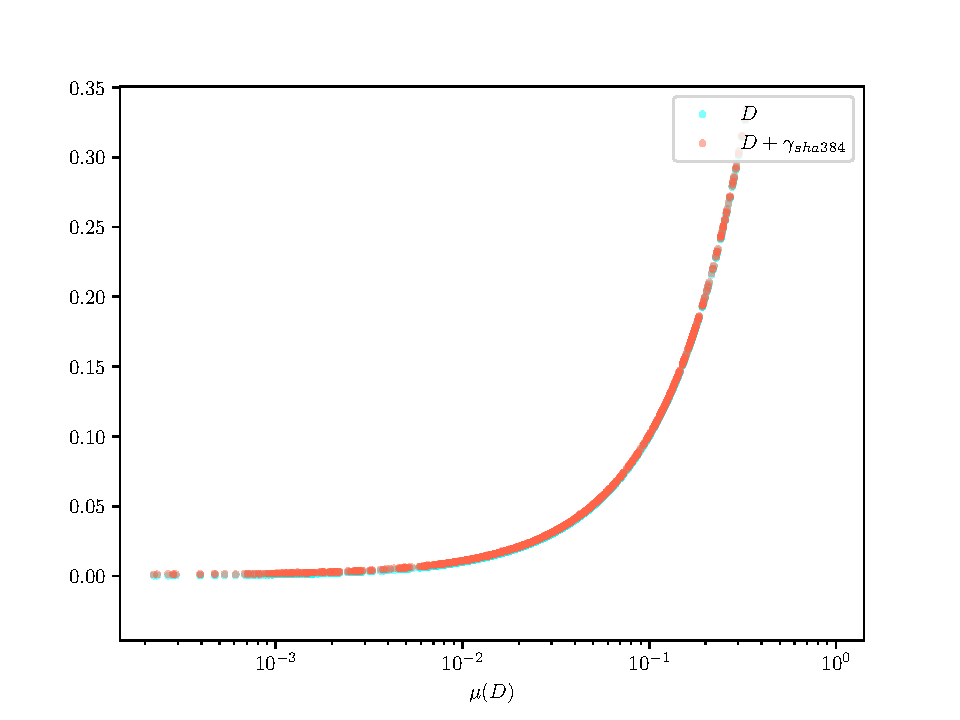
\includegraphics[width=\linewidth]{figures/stat_sha384_0mean.pdf}
				\caption{mean}
			\end{subfigure}
			\begin{subfigure}{0.32\linewidth}
				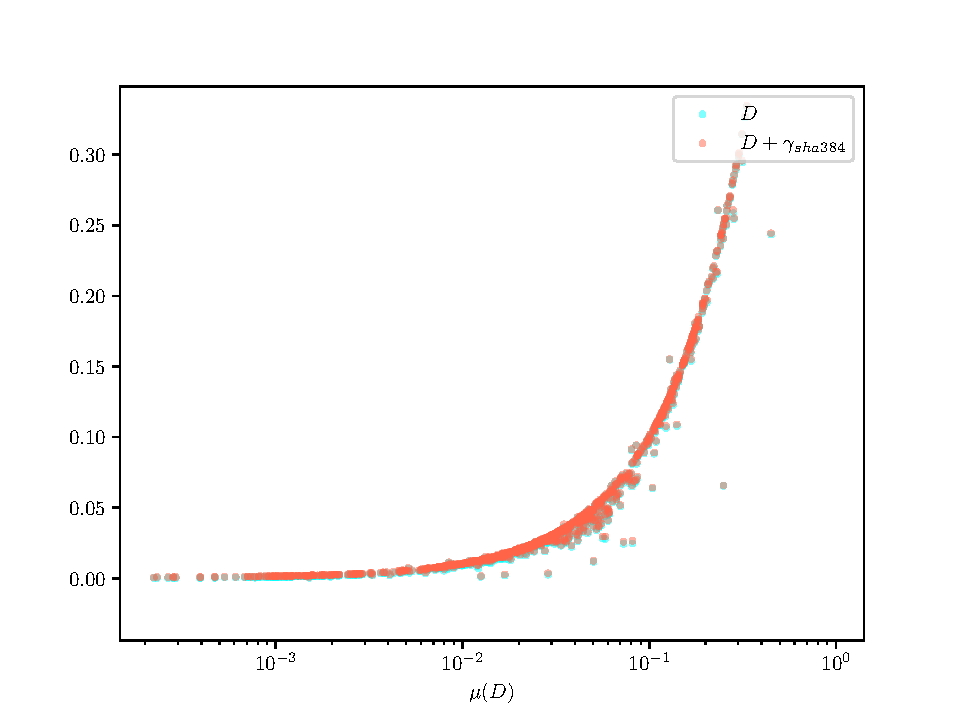
\includegraphics[width=\linewidth]{figures/stat_sha384_0median.pdf}
				\caption{median}
			\end{subfigure}
			\begin{subfigure}{0.32\linewidth}
				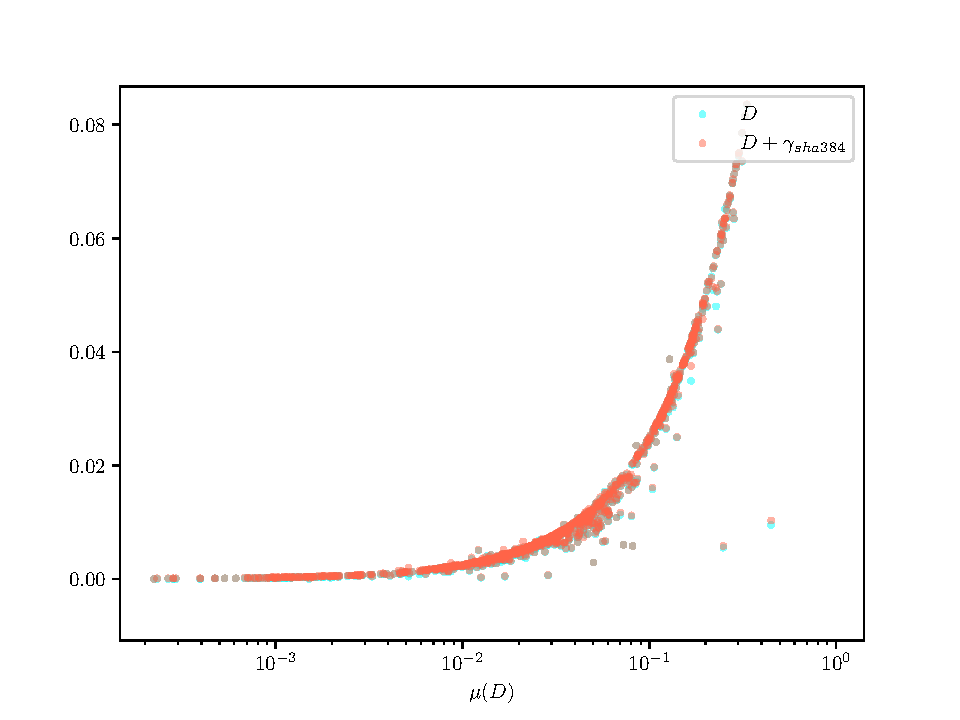
\includegraphics[width=\linewidth]{figures/stat_sha384_0mode.pdf}
				\caption{mode}
			\end{subfigure}
			\begin{subfigure}{0.32\linewidth}
				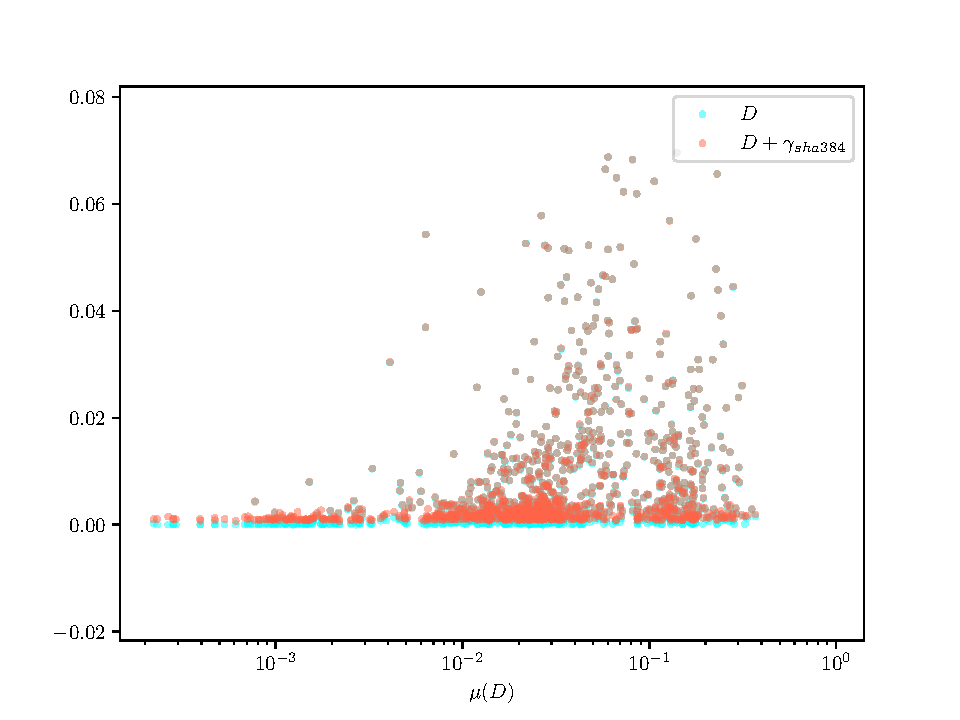
\includegraphics[width=\linewidth]{figures/stat_sha384_0std.pdf}
				\caption{standard deviation}
			\end{subfigure}
			\begin{subfigure}{0.32\linewidth}
				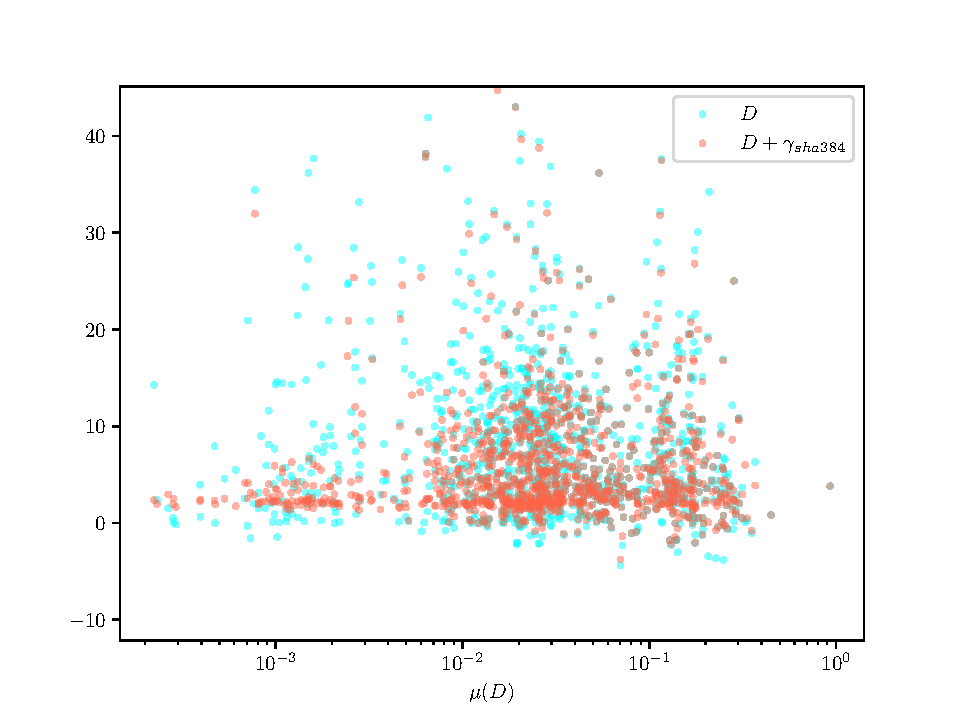
\includegraphics[width=\linewidth]{figures/stat_sha384_0skew.pdf}
				\caption{skewness}
			\end{subfigure}
			\begin{subfigure}{0.32\linewidth}
				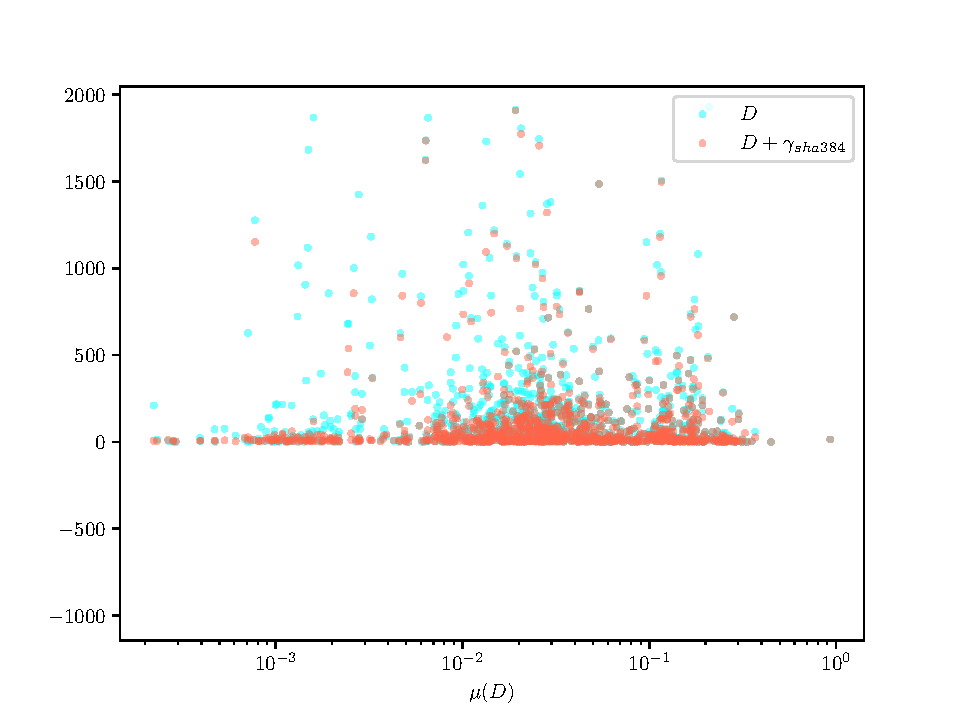
\includegraphics[width=\linewidth]{figures/stat_sha384_0kurtosis.pdf}
				\caption{kurtosis}
			\end{subfigure}
			\begin{subfigure}{0.32\linewidth}
				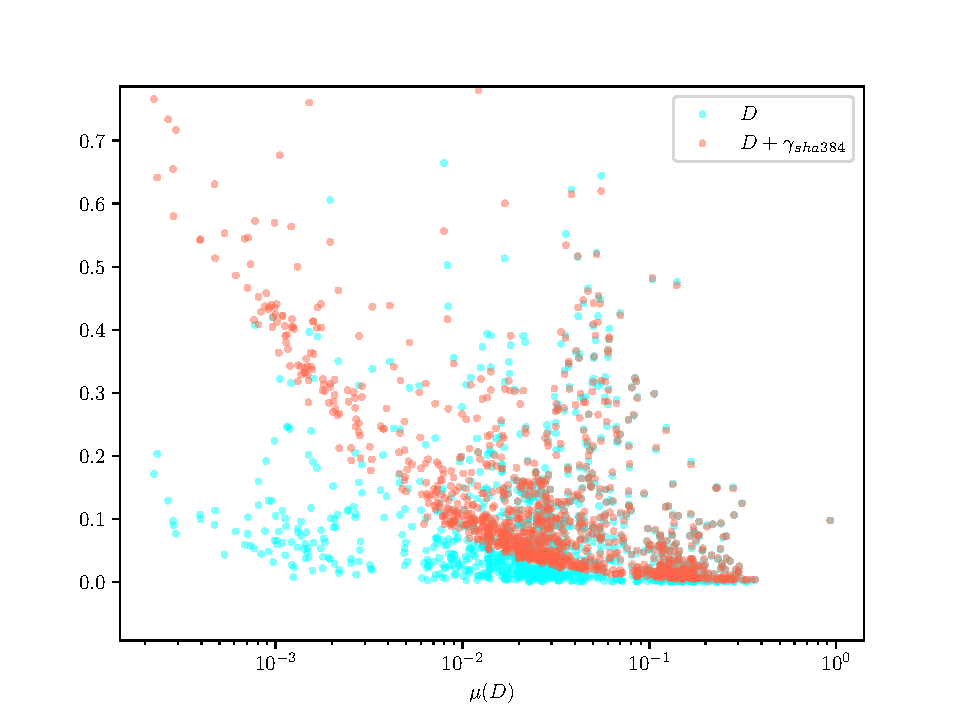
\includegraphics[width=\linewidth]{figures/stat_sha384_0hill_est.pdf}
				\caption{Hill\\tail estimator}
			\end{subfigure}
			\begin{subfigure}{0.32\linewidth}
				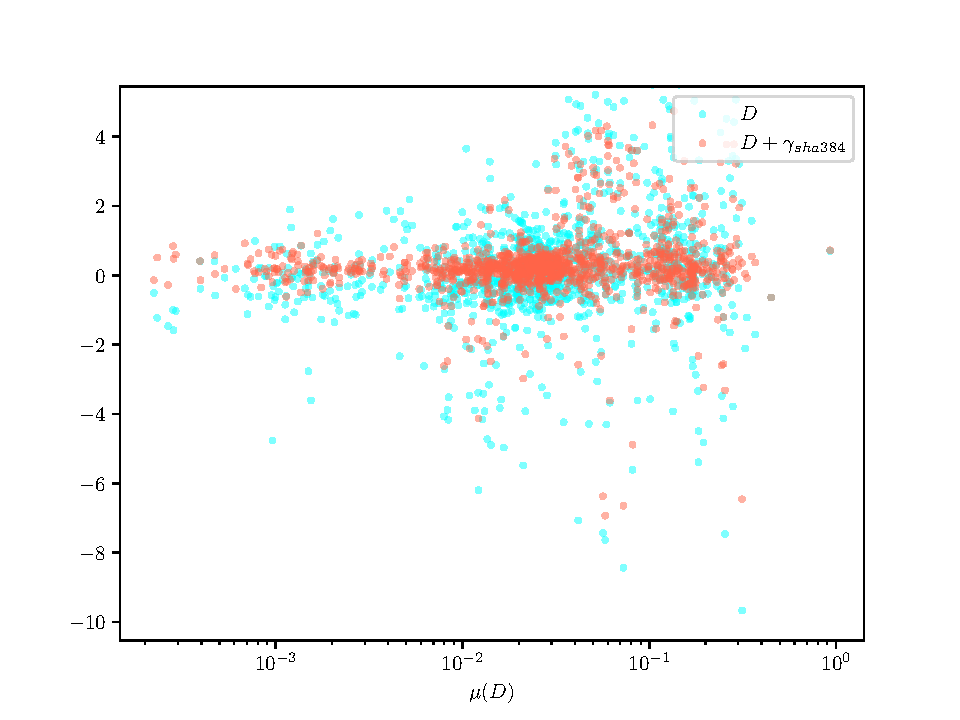
\includegraphics[width=\linewidth]{figures/stat_sha384_0pickands_est.pdf}
				\caption{Pickands\\tail estimator}
			\end{subfigure}
			\begin{subfigure}{0.32\linewidth}
				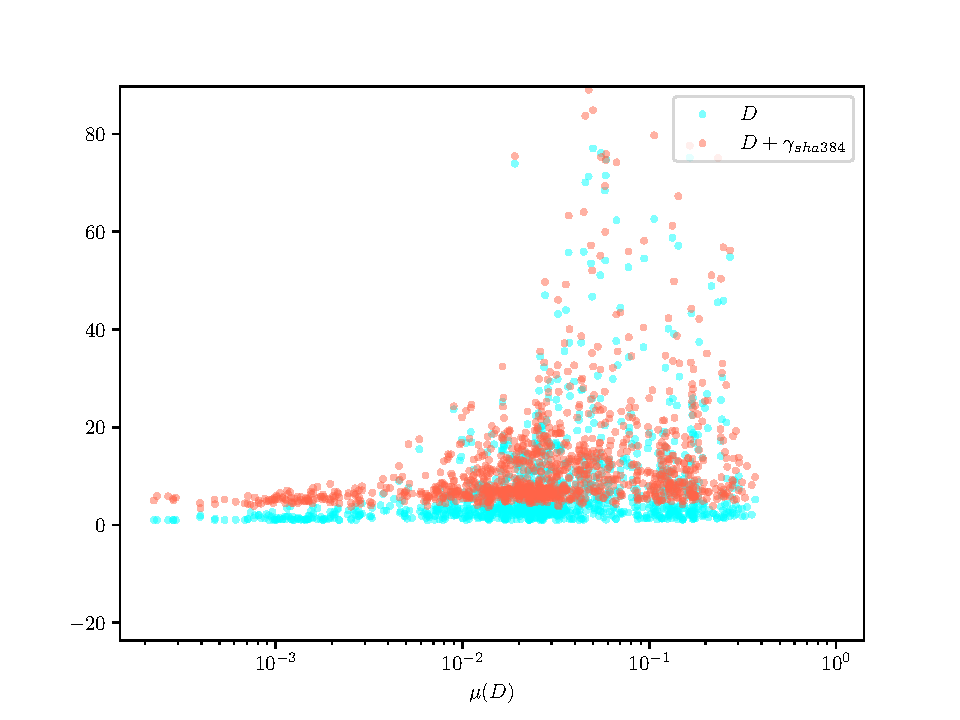
\includegraphics[width=\linewidth]{figures/stat_sha384_0suessmann.pdf}
				\caption{Süssmann\\measure}
			\end{subfigure}
			\begin{subfigure}{0.32\linewidth}
				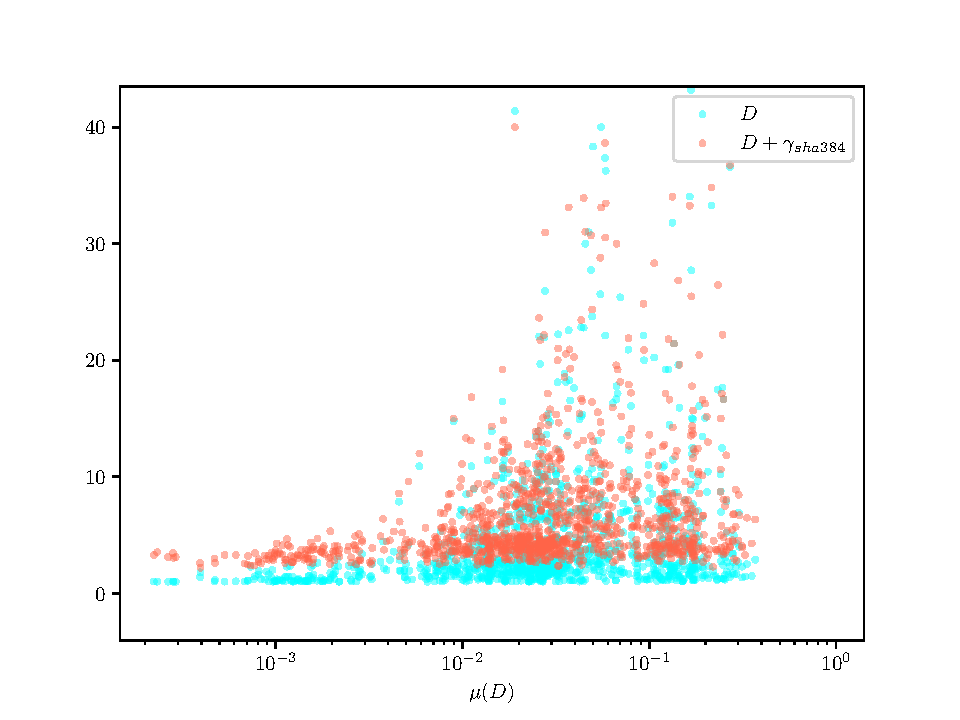
\includegraphics[width=\linewidth]{figures/stat_sha384_0max_hist_inverse.pdf}
				\caption{reciprocal of \\maximum histogram value}
			\end{subfigure}
			\begin{subfigure}{0.32\linewidth}
				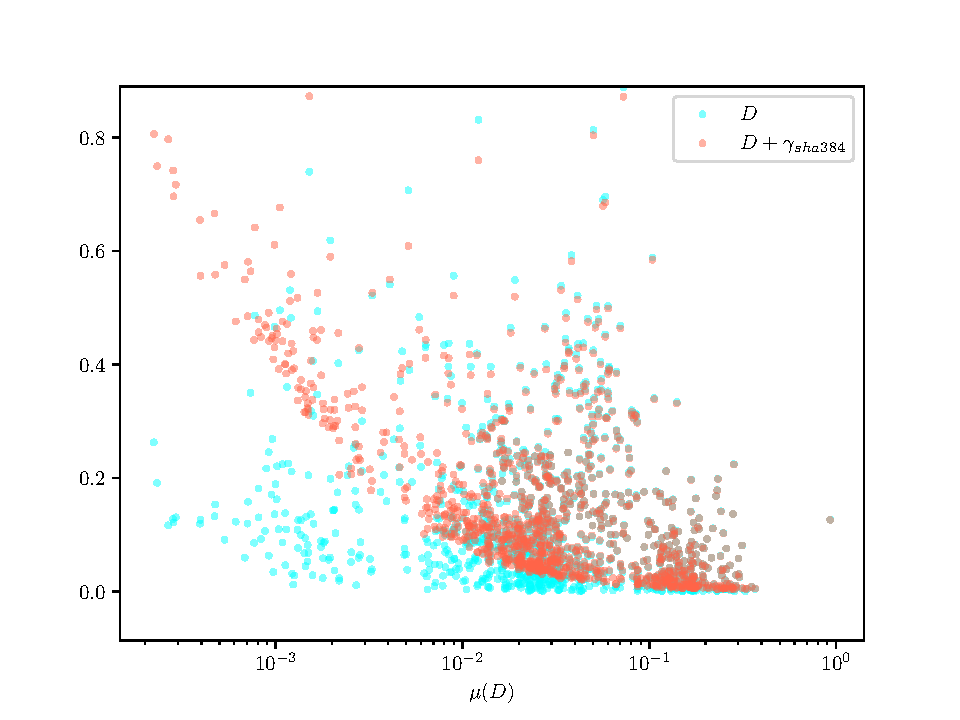
\includegraphics[width=\linewidth]{figures/stat_sha384_0log_std.pdf}
				\caption{standard deviation \\of logarithm}
			\end{subfigure}
			\begin{subfigure}{0.32\linewidth}
				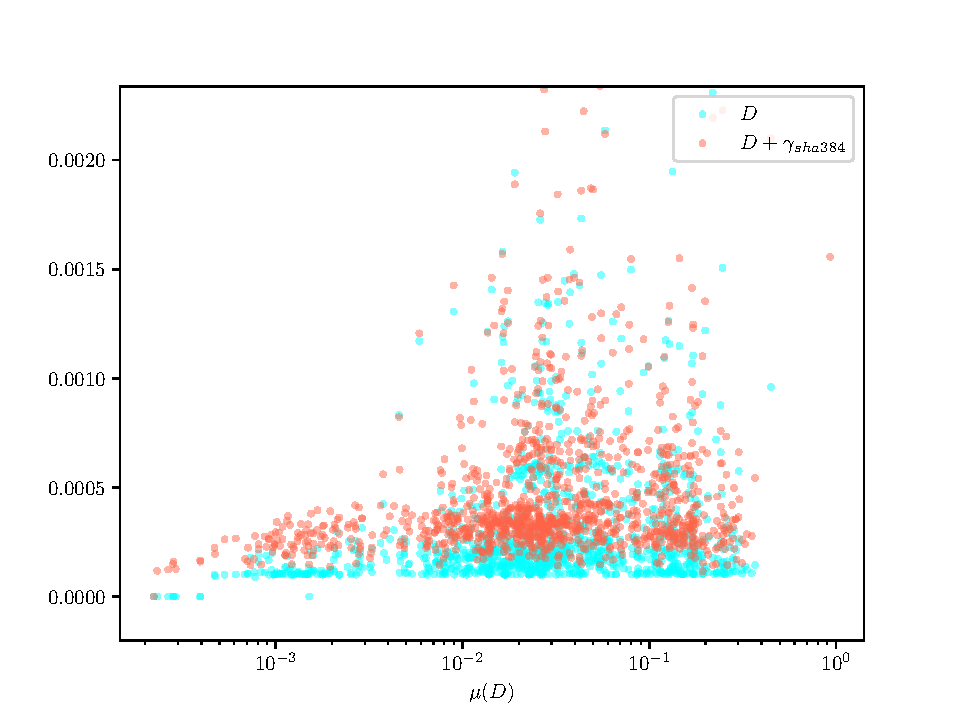
\includegraphics[width=\linewidth]{figures/stat_sha384_0FWHM.pdf}
				\caption{FWHM of\\maximum peak}
			\end{subfigure}
		\begin{subfigure}{0.32\linewidth}
			\hphantom{a}
		\end{subfigure}
			\caption{Values of $\alpha(D)$ (blue) and $\alpha(D + \gamma_{sha384})$ (red) for various statistical measures $\alpha$ plotted against $\mu(D)$ for data from the RIPE Atlas dataset}
			\label{stat-mes-fig-2}
		\end{figure}%
	%
	%
		\begin{figure}
		\begin{subfigure}{0.32\linewidth}
			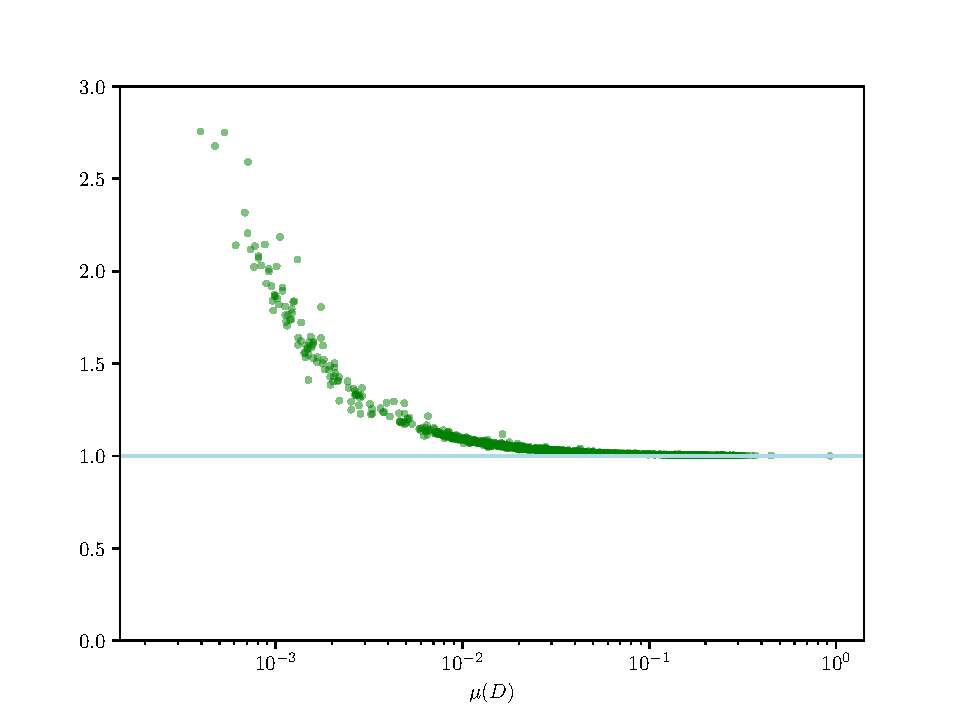
\includegraphics[width=\linewidth]{figures/stat_sha384_0mean_div.pdf}
			\caption{mean}
		\end{subfigure}
		\begin{subfigure}{0.32\linewidth}
			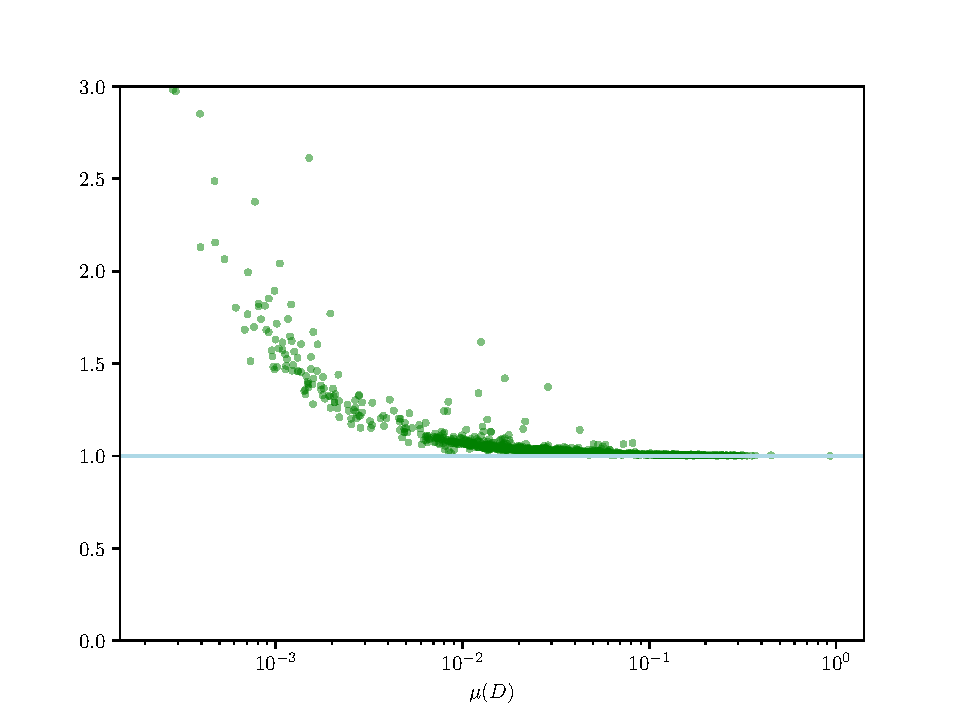
\includegraphics[width=\linewidth]{figures/stat_sha384_0median_div.pdf}
			\caption{median}
		\end{subfigure}
		\begin{subfigure}{0.32\linewidth}
			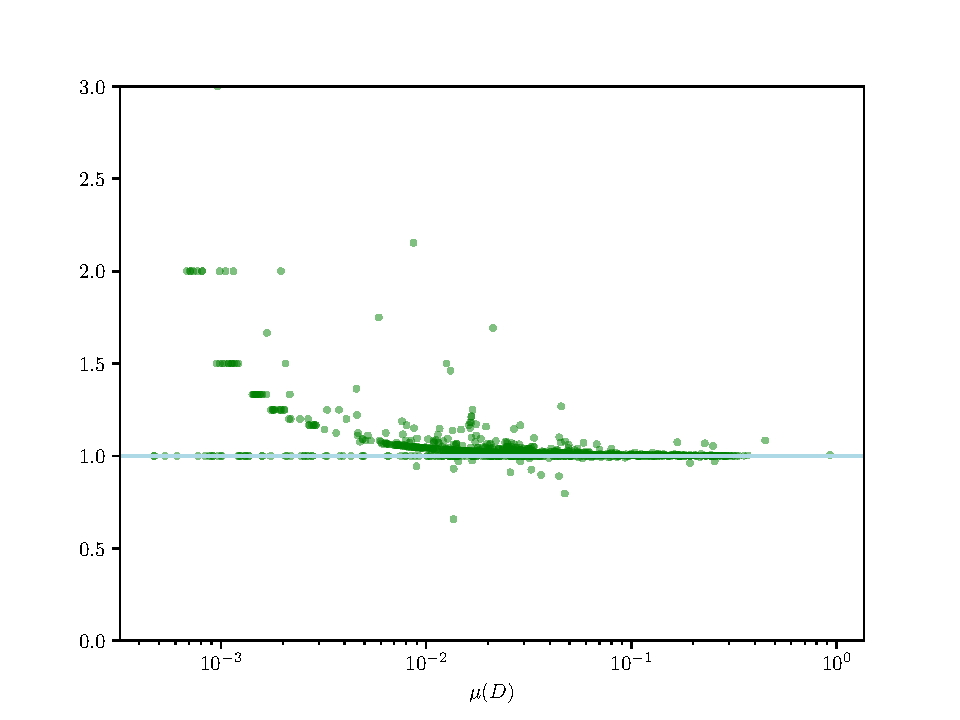
\includegraphics[width=\linewidth]{figures/stat_sha384_0mode_div.pdf}
			\caption{mode}
		\end{subfigure}
		\begin{subfigure}{0.32\linewidth}
			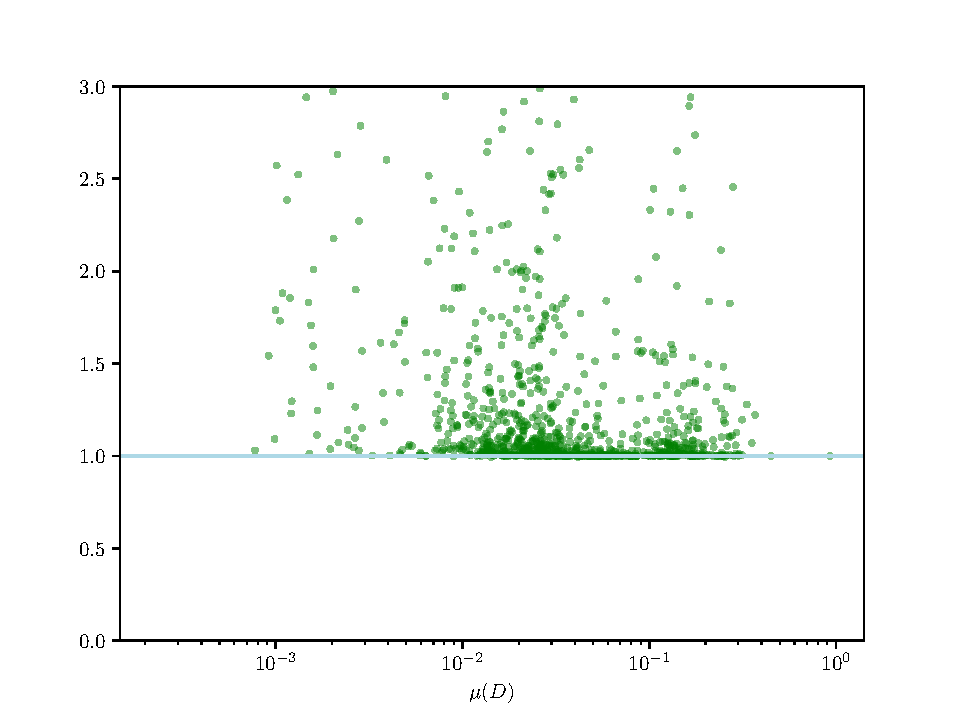
\includegraphics[width=\linewidth]{figures/stat_sha384_0std_div.pdf}
			\caption{standard deviation}
		\end{subfigure}
		\begin{subfigure}{0.32\linewidth}
			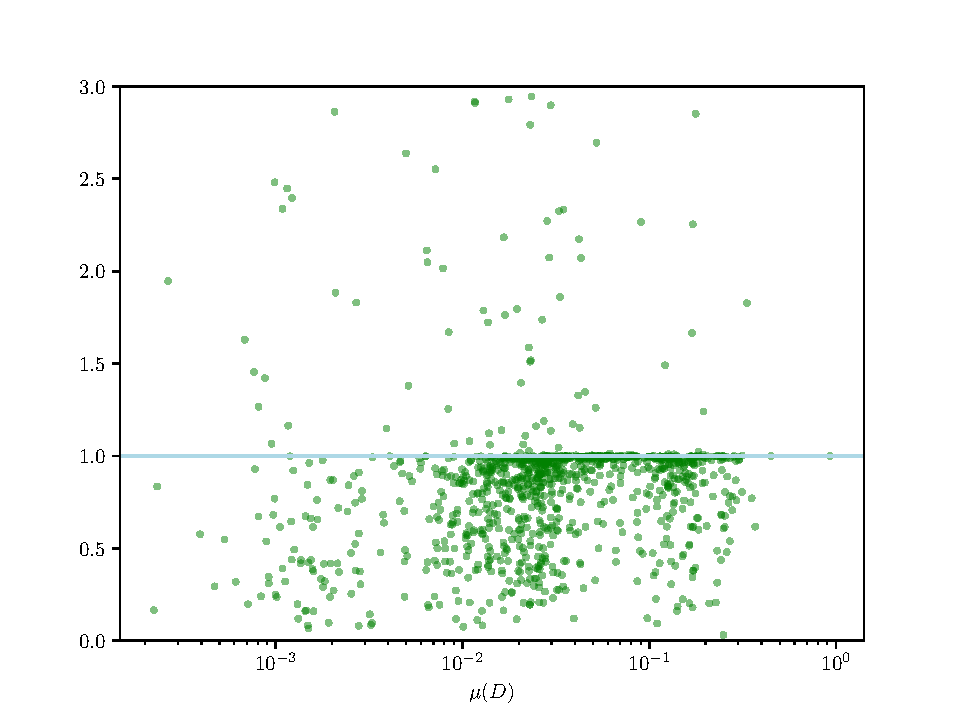
\includegraphics[width=\linewidth]{figures/stat_sha384_0skew_div.pdf}
			\caption{skewness}
		\end{subfigure}
		\begin{subfigure}{0.32\linewidth}
			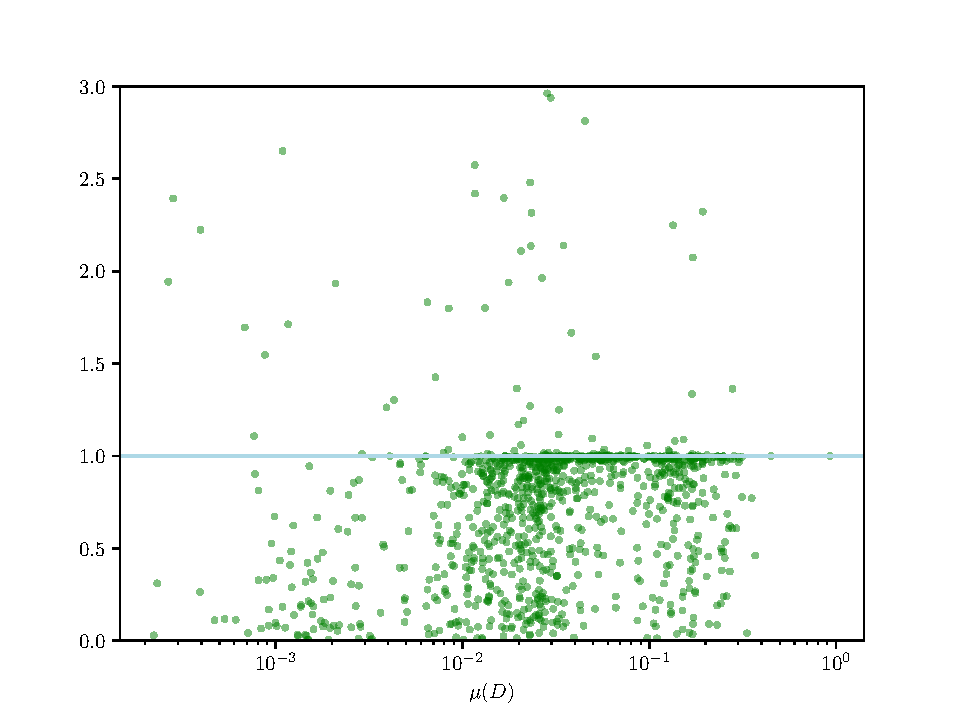
\includegraphics[width=\linewidth]{figures/stat_sha384_0kurtosis_div.pdf}
			\caption{kurtosis}
		\end{subfigure}
		\begin{subfigure}{0.32\linewidth}
			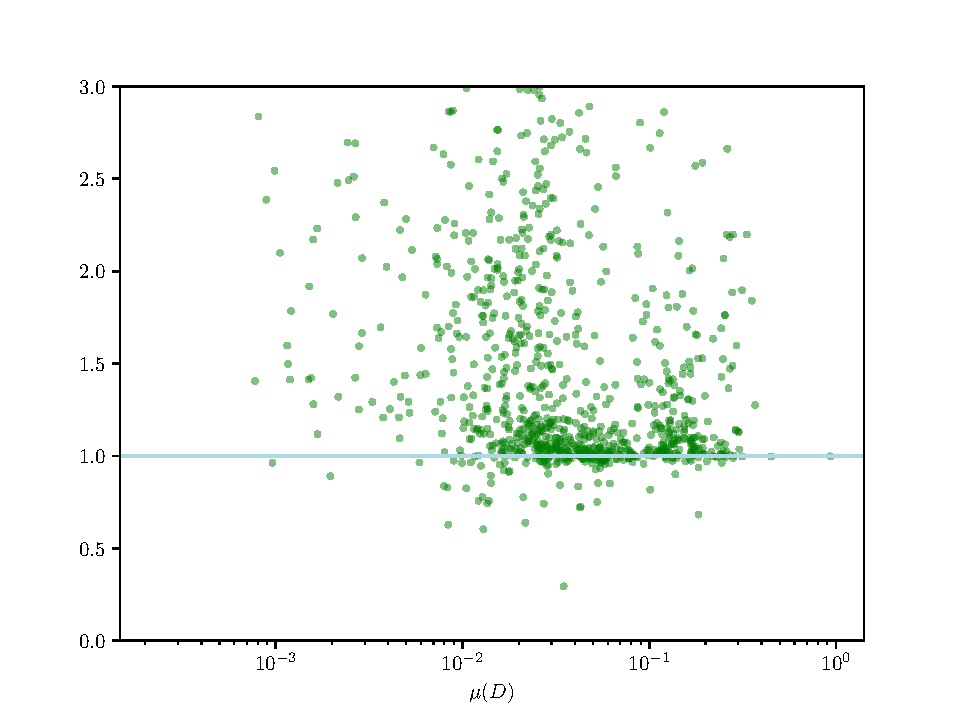
\includegraphics[width=\linewidth]{figures/stat_sha384_0hill_est_div.pdf}
			\caption{Hill\\tail estimator}
		\end{subfigure}
		\begin{subfigure}{0.32\linewidth}
			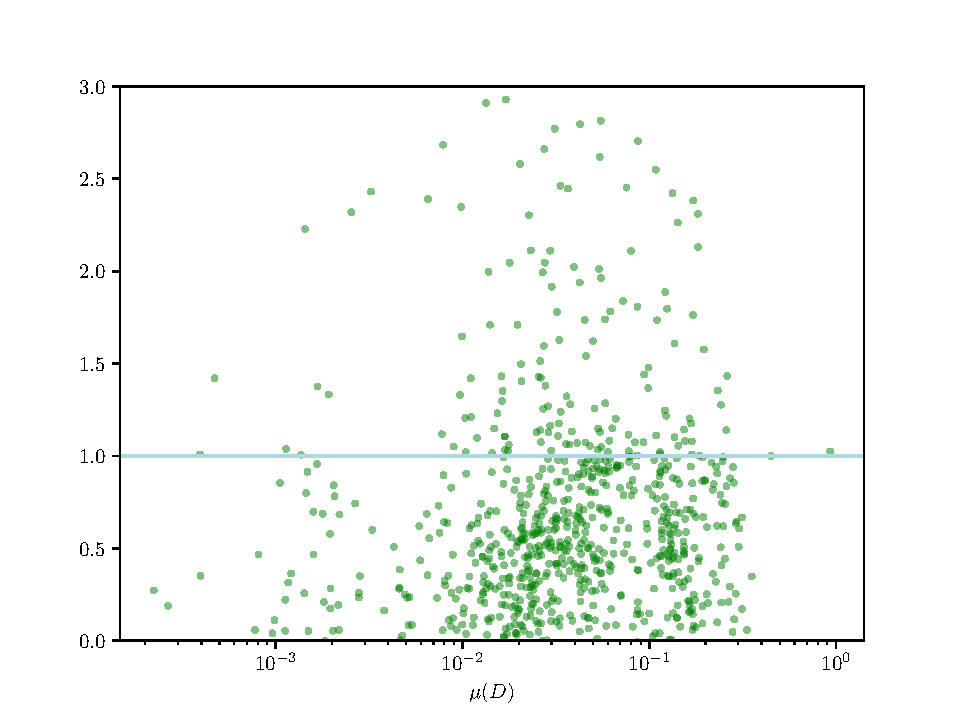
\includegraphics[width=\linewidth]{figures/stat_sha384_0pickands_est_div.pdf}
			\caption{Pickands\\tail estimator}
		\end{subfigure}
		\begin{subfigure}{0.32\linewidth}
			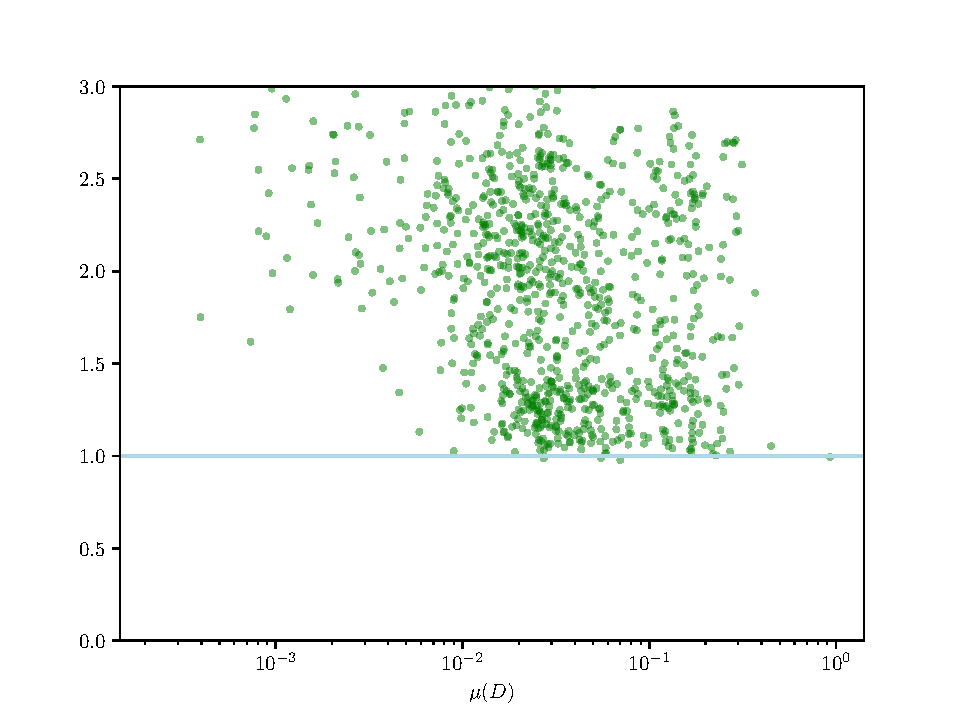
\includegraphics[width=\linewidth]{figures/stat_sha384_0suessmann_div.pdf}
			\caption{Süssmann\\measure}
		\end{subfigure}
		\begin{subfigure}{0.32\linewidth}
			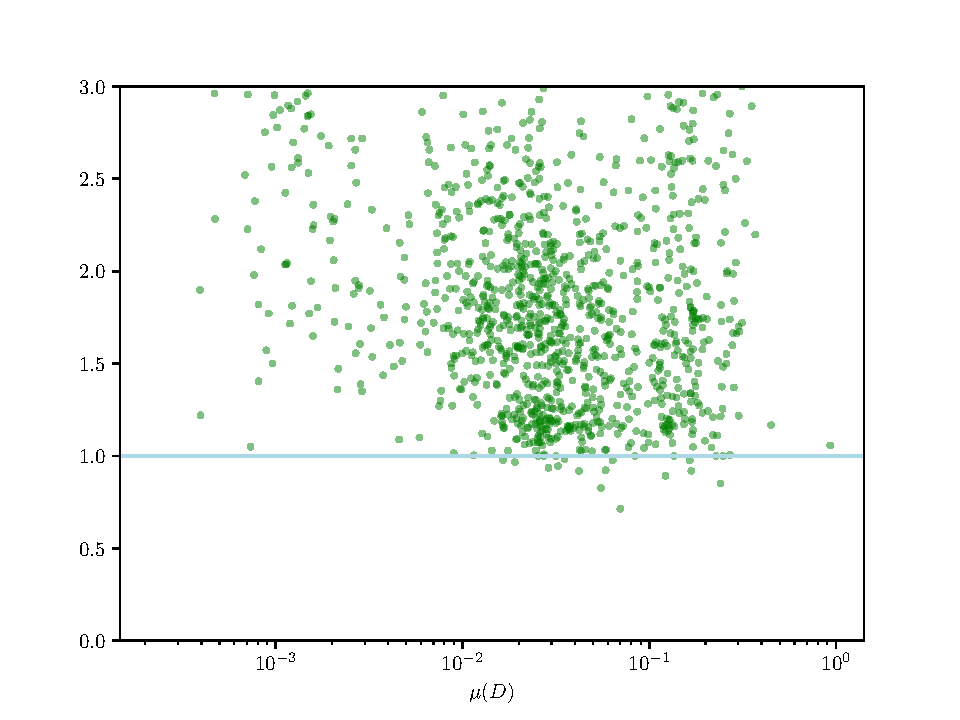
\includegraphics[width=\linewidth]{figures/stat_sha384_0max_hist_inverse_div.pdf}
			\caption{reciprocal of\\maximum histogram value}
		\end{subfigure}
		\begin{subfigure}{0.32\linewidth}
			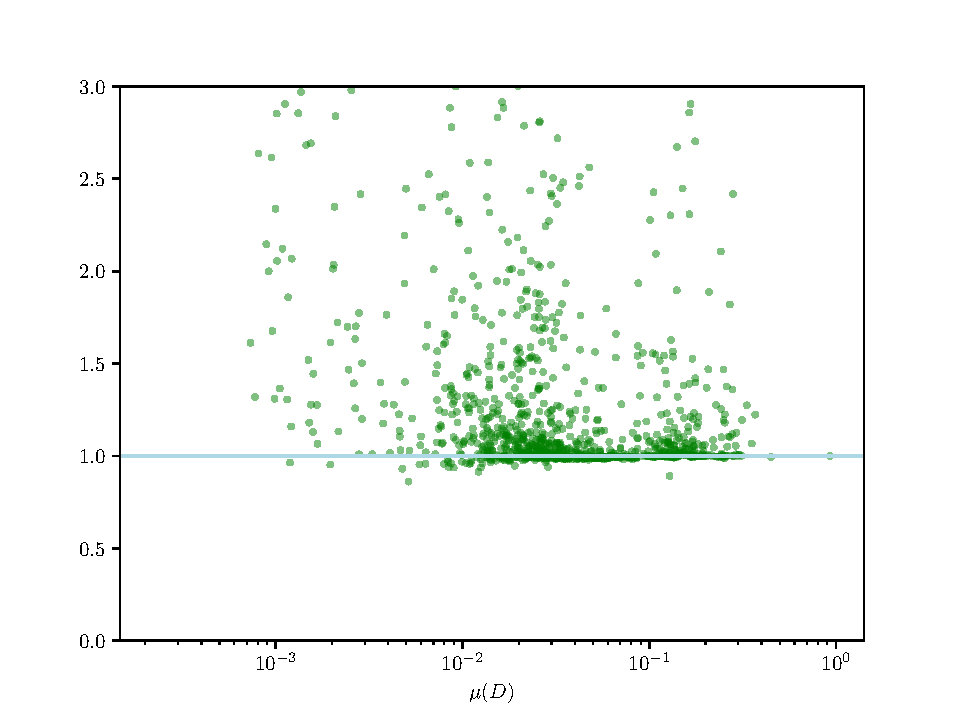
\includegraphics[width=\linewidth]{figures/stat_sha384_0log_std_div.pdf}
			\caption{standard deviation\\of logarithm}
		\end{subfigure}
		\begin{subfigure}{0.32\linewidth}
			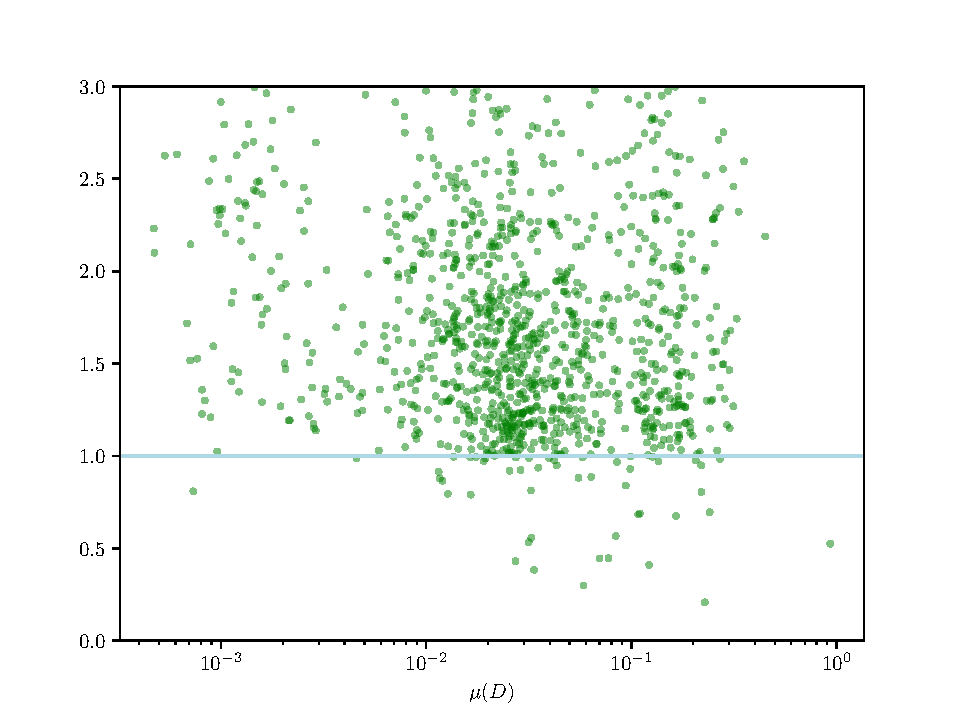
\includegraphics[width=\linewidth]{figures/stat_sha384_0FWHM_div.pdf}
			\caption{FWHM of\\maximum peak}
		\end{subfigure}
		\begin{subfigure}{0.32\linewidth}
			\hphantom{a}
		\end{subfigure}
		\caption{Ratio of $\alpha(D)$ to $\alpha(D + \gamma_{sha384})$ for various statistical measures $\alpha$ plotted against $\mu(D)$ for data from the RIPE Atlas dataset. Light blue line is plotted at $y=1$}%
		\label{stat-mes-fig}%
	\end{figure}
			Figure \ref{stat-mes-fig-2} shows the values of these statistical measures for $D$ and $D + \gamma$ with $\gamma$ for a hash-chain covert channel using the sha384 hash algorithm for all connections in the RIPE Atlas dataset, plotted against the average latency of the connection. Figure \ref{stat-mes-fig} shows the ratio $\frac{\alpha(D + \gamma)}{\alpha(D)}$.
			We can observe in \ref{stat-mes-fig} (a)-(c) that the central measures mean, median and mode follow a hyperbolic curve, as is expected, because $\frac{\mu(D + \gamma)}{\mu(D)}$ approximates to $1 + \frac{\mu(\gamma)}{\mu(D)}$.
			
			\pagebreak
			
			Based on these results it seems sensible to try a threshold based detection approach using some of these statistical metrics. For a metric $\alpha$ we can define some threshold $t_\alpha$ with $\mu_\alpha(D) < t_\alpha < \mu_\alpha(D+\gamma)$ or $\mu_\alpha(D) > t_\alpha > \mu_\alpha(D+\gamma)$ with $\mu_\alpha(X)$ being the average value of $\alpha$ for the dataset $X$. The most straightforward approach would be choosing $t_\alpha = \frac{\mu_\alpha(D) + \mu_\alpha(D + \gamma)}{2}$. We can now define a decision function:
			\begin{equation}
				\label{thresh-equ}
				f_\alpha(D^*) = 
				\begin{cases}
					1 & \text{if } C(\alpha(D^*), t_\alpha) \\
					0 & \text{otherwise}
				\end{cases}
			\end{equation} 
			where $C(x, y)$ is a comparison operator. If $\mu_\alpha(D) < \mu_\alpha(D + \gamma)$ then $C(\alpha(D^*), t_\alpha) = \alpha(D^*) > t_\alpha$; if $\alpha(D^*) > t_\alpha$, if $\mu_\alpha(D) > \mu_\alpha(D + \gamma)$ then $C(\alpha(D^*), t_\alpha) = \alpha(D^*) < t_\alpha$. \\
			Because $\gamma > 0$ it follows in general that $c(D + \gamma) > c(D)$ for a central measure $c$ (mean, median or mode). We can now define a straightforward specific mean threshold decision function $f_c(D^*)$. The choice of $c$ depends on context. Mean and Median behave similarly as can be seen in figure \ref{stat-mes-fig} (a) and (b), however the median possesses greater protection against outliers that are to be expected when working with heavy tailed distributions. The mean on the other hand should produce more reliable results for smaller window sizes, as it is able to change more dynamically than the median. The mode can provide additional certainty for large window sizes when the latency distribution possesses sharp, singular peaks (e.g. figure \ref{comparison-fig} (c)), it should however in general be avoided as it is possible for $mode(D+\gamma) < mode(D)$ when dealing with particularly flat distributions (e.g. the bottom figure of \ref{comparison-fig} (d)). \\
			Because $c(D)$ will vary over time, any implementation of $f_c$ will have to modify $t_c$ based on changing network properties and continuously updated latency measurements. To gauge the potential of $f_c$, we can compare the standard deviation of $D$ with the mean of $\gamma$ (c.f. figure \ref{mean-fig}). We can observe that around $\mu(D) \approx 10^{-2} s$ both $\sigma(D) \approx \mu(\gamma)$ as well as $\frac{\mu(\gamma)}{\mu(D)} \approx 10\%$ (c.f. figure \ref{stat-mes-fig} (a)). This indicates a lower success rate for $f_\alpha$ decision functions in general and $f_c$ functions specifically, because random changes of the variable and $\gamma$ are of the same magnitude\footnote{This ignores the effect of seasonality and concept drift on $D$ which can further increase its variance and cause threshold detection with central measures to fail for these datasets. These effects can be observed the most clearly in the changes of the lan dataset in figure \ref{comparison-fig} (a)}. \\
			The Mann-Whitney U Test  \cite{Mann1947} is used to determine whether one random variable $X$ is statistically bigger than another random variable $Y$ without making assumptions about their specific distributions. This helps us gauge the general detectability of $\gamma$ based on measures of centrality and scale. It works by calculating $U$ from a sample of $n$ values of $X$ and $m$ values of $Y$: \begin{equation}
				U = \sum_{i=1}^{n}\sum_{j=1}^{m}S(X_i, Y_j)
			\end{equation}
			with 
			\[
			S(X, Y) = \begin{cases}
				1 & \text{if } X>Y\\
				\frac{1}{2} & \text{if } X=Y\\
				0 & \text{if } X<Y
			\end{cases}.
			\]
			We can now treat U as a normally distributed variable and apply standard hypothesis tests to determine a $\rho$-value against the Null-Hypothesis $X<Y$. This value can be used as a measure of minimum differentiability between $D$ and $D+\gamma$. We say that two samples $X$ and $Y$ are significantly differentiable if $\rho<0.05$. Figure \ref{mwu-fig} shows the percentage of significant Mann-Whitney U $\rho$-values when taking 25 random samples of size 50 from $D$  and $D+\gamma$ for connections from the RIPE Atlas dataset. At $\mu(D) \approx 10^{-2} s$ a significant drop-off in  differentiability can be observed, this is consistent with the previous observations from figure \ref{mean-fig}.\\
			In order to characterize this drop-off, we have arbitrarily split the RIPE Atlas dataset along $\mu(D)=20ms \approx 10^{-2} s$ and calculated the cumulative differentiability for both halves of the dataset. The results can be seen in table \ref{mwu-tab} and roughly reflect the probability that a covert channel using the given hash function can be detected on a random connection by looking at windows of size 50. This can be taken as a measure of the maximum accuracy of central measure threshold tests. \\
			\begin{figure}
				\centering
				\begin{subfigure}{0.48\linewidth}
					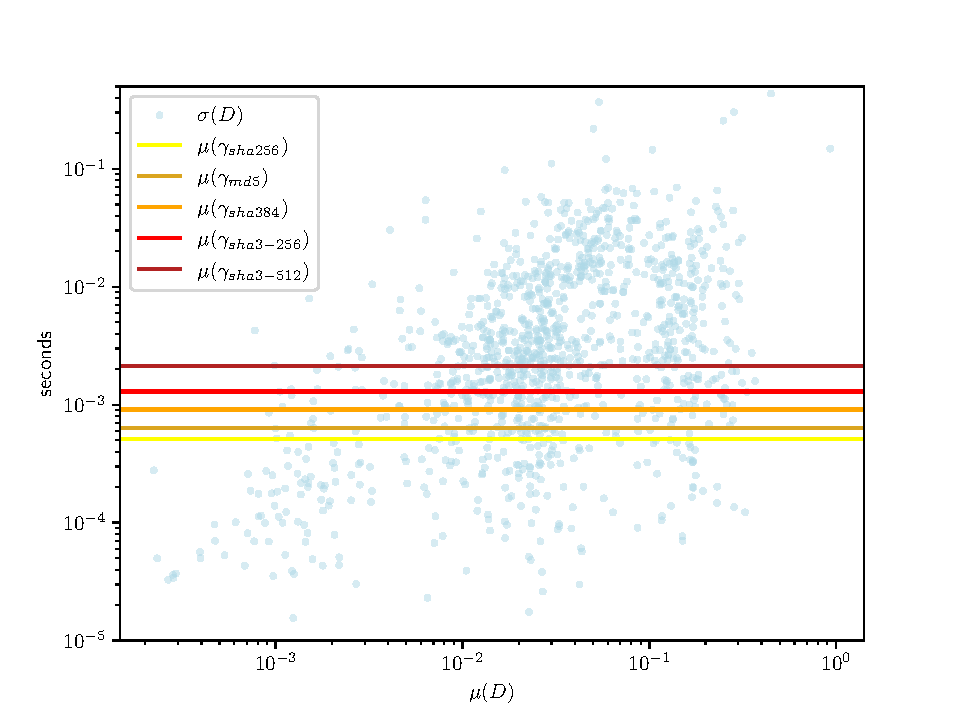
\includegraphics[width=\linewidth]{figures/stat_md5_0std_diff.pdf}
					\caption{RIPE Atlas dataset}
				\end{subfigure}
				\begin{subfigure}{0.48\linewidth}
					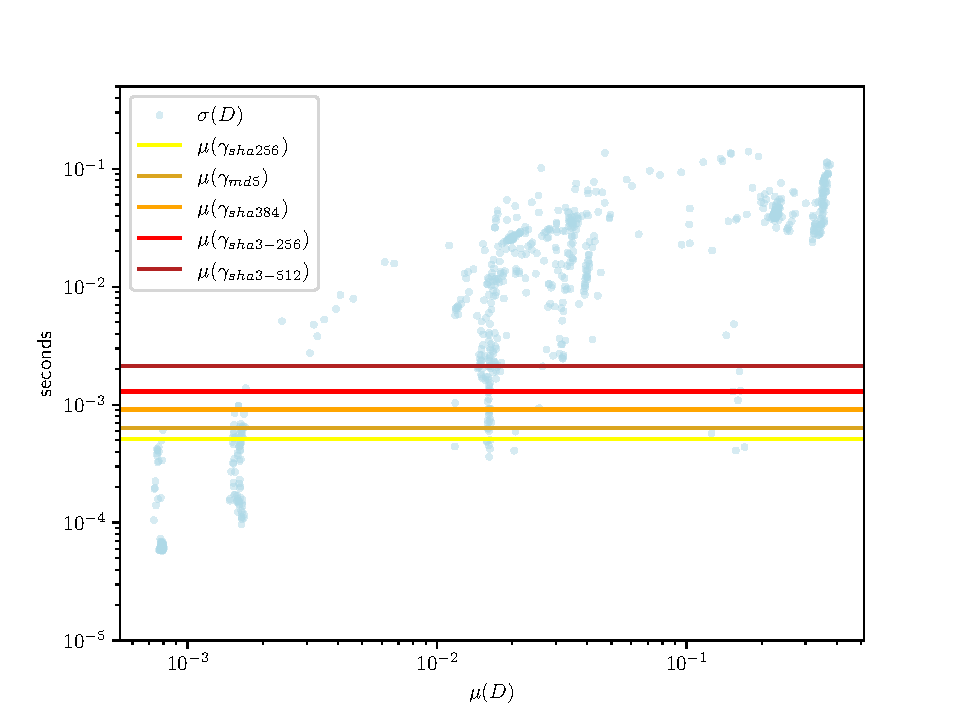
\includegraphics[width=\linewidth]{figures/stat_md5_00all_std_diff.pdf}
					\caption{self-made measurements}
				\end{subfigure}
				\caption{Comparison of standard deviation for connections and mean values of simulated covert channel delays}
				\label{mean-fig}
			\end{figure}
			\begin{figure}
				\centering
				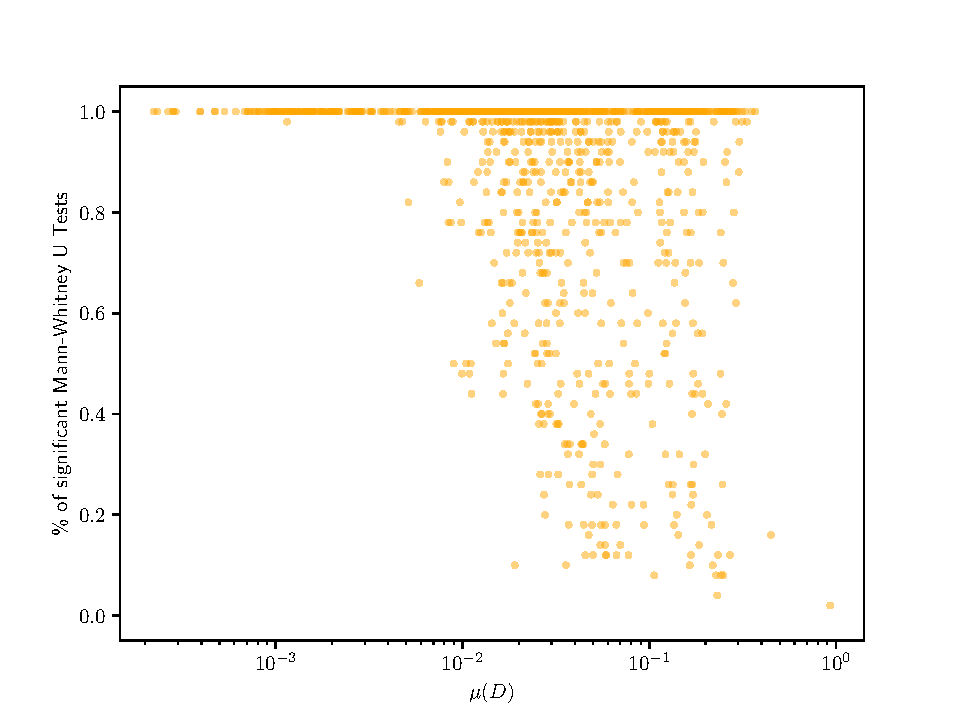
\includegraphics[width=0.4\linewidth]{figures/mwu_p_50__sha384_0.pdf}
				\caption{Percentage of significant Mann-Whitney U Tests for random samples of size 50 from $D$ and $D+\gamma_{sha384}$}
				\label{mwu-fig}
			\end{figure}
			\begin{table}
				\centering
					\begin{tabular}{l | l | l | l | l }
						$n$ & sha256 & md5 & sha384 & sha3-256\\ % & sha3-512 \\
						\hline
						$\mu(D) < 20 ms$ &  90\% & 93\% & 95\% & 98\%  \\
						$\mu(D) \geq 20 ms$ & 73\% & 76\% & 83\% & 89\%  \\
					\end{tabular}
			\caption{Percentage of significant Mann-Whitney U tests by hash function for random samples of size 50 from $D$ and $D+\gamma$ (sha3-512 not included as we did not simulate covert channels using this hash algorithm for the RIPE Atlas dataset)}
			\label{mwu-tab}
			\end{table}
			We may be able to detect $\gamma$ with even higher accuracy by measuring its effect on the peak width and tail heaviness of $D^*$. Similar to $f_c$, we can define a specific decision function $f_\omega$ based on some measure of shape $\omega$.
			\pagebreak\\ 
			For standard deviation (d), skewness (e) and kurtosis (f), we can observe that while for many connections a drastic change occurs between $D$ and $D + \gamma$, this change is universal and, for skewness and kurtosis, not unidirectional. While the Pickands estimator also performs rather poorly (c.f. figure \ref{stat-mes-fig-2} (h)), the other shape metrics produce promising results and could be used for this purpose. For the Hill estimator(g) and the standard deviation of the logarithm (k) we can see a clear separation between $D$ and $D + \gamma$ for low latencies. For the Süssmann measure (i), the reciprocal of the maximum histogram value (j) and the peak width (l), we can observe that there exists a threshold below which only data points from $D$ can be observed (c.f. figure \ref{stat-mes-fig-2}), making them a great candidate for a threshold measure $\omega$. All these metrics increase significantly even for high latency connection when $\gamma$ is added to $D$ (c.f. figure \ref{stat-mes-fig}). Whether these values are more resistant to concept drift and seasonality than measures of centrality remains and open question for further research.\\
			A combination of $f_c$ and $f_\omega$ could also be used to grant greater protection against modified alphabets. The optimal alphabet $L_0$ (On which the plots in figures \ref{comparison-fig} and \ref{stat-mes-fig} are based) is easier caught by $f_\omega$ than $f_c$. An attacker could modify $L$ or normalize latency in order to reduce the impact of the covert channel on peak width, this would however increase overall latency, which could be picked up by $f_c$.
		\section{Possible Machine Learning Usage}
		\label{ens-stat}
			
			
			Machine learning possesses the ability to accurately classify data based on very complex relations between input variables and can be used to accurately approximate computationally intensive calculations \cite{ml_web1}. Such algorithms also have the inherent advantage, that they can be directly trained on previously captured data or simulated versions of reversible covert channels similar to those used in this thesis. This enhances its protective capabilities against modified alphabets as well as normalized delay and even other kinds of computationally intensive covert channel.\\
			However, machine learning often comes with a high initial planning and computational cost. For the classification of data streams many machine learning models also would need to be adjusted and trained continuously in order to avoid concept drift, leading to lower performance. One can find many examples of machine learning not significantly outperforming classical statistical models when the relationship between input variables and their classification isn't particularly complex \cite{Christodoulou2019}. 
			\pagebreak\\
			In order for machine learning classification of $D^*$ to outperform traditional statistical approaches, one of the following conditions needs to hold true:
			
			\begin{enumerate}
				\item It is possible to differentiate $D$ from $D + \gamma$ using some set of statistical measures $S$. The classification function 
				\begin{equation}
					f_S(D^*)=\begin{cases}
						0,				& \text{if } D^* = D\\
						1,              & \text{if } D^* = D + \gamma
					\end{cases}
				\end{equation}
				however has no easily definable and generalizable form or changes dramatically based on the properties of $D$. This would open up the possibility of a machine learning algorithm being able to learn this complex pattern, while a normal statistical model would not be able to portray it accurately.
				\item There exists a representation of $D^*$ (e.g. empirical probability distribution) that enables a machine learning algorithm to take advantage of complex but easily classifiable relations on this representation in order to classify $D^*$ more accurately / faster than statistical approaches.
				\item When the temporal ordering is taken into account, the covert channel can be detected more easily. Most statistical approaches will discard the temporal ordering of analysed series and thus be blind to potential temporal clues
			\end{enumerate}
			
			We will ignore the last possibility in this thesis as it is quite unlikely that viewing $D^*$ as anything other than a random variable is going to help us differentiate $D$ from $D + \gamma$. This is the case because, as we have argued in section \ref{network-lat}, both $D$ and $\gamma$ can essentially be modelled as random variables. We still performed preliminary research with temporal convolutional kernel and Fourier decomposition based machine learning approaches on the raw time series data with very little success.\\
			The first possibility lends itself very well to algorithms based on decision trees, as these are implemented via a complex series of binary decisions, which is well suited to differentiating statistical data. We tested regular simple Decision Tree as well as Random Forest algorithms, which both classify the data by building one or multiple binary trees from splitting points in the training data. Classifier boosting refers to building an ensemble classifier from copies of a base classifier which are trained with a focus on difficult parts of the data set. GradientBoost and AdaBoost are two such boosting classifiers which are usually build using instances of decision tree classifiers \cite{Pedregosa2011}. 
			We also tested Gaussian Naive Bayes, logistic regression, ridge regression and support vector machine algorithms. These algorithms are good at modelling various types of linear or polynomial relationships between variables. Because of the non-linear nature of the statistical measurements included in our set $S$ as well as the suitability of binary decisions for the classification of a small set of statistical measures, most of these models were not able to compete with decision trees, as will be seen in section 4.2. \\
			There are a lot of possible ways to tackle the second possibility of detection. Any graphical statistical analysis method could be used as a basis for a less processed representation of the connection measurements. We have chosen to focus on the shape of the resulting empirical probability distribution as indicator of the presence of $\gamma$. Our algorithm will generate a fine-grain normalized histogram of the input measurements and treat it as a signal or 1-dimensional image to perform image recognition. The core idea behind this implementation is that while the exact way in which the shape of the distribution changes could be very difficult to describe mathematically, we can train a image recognition model to pick up on the subtle differences between modified and unmodified probability functions.\\
			Convolutional neural networks are well suited for this tasks, as they are particularly good at picking up on complex relationships in abstract sets of data.  This has the potential for higher efficiency and greater scalability. Similar to  \cite{Al-Eidi2021} and \cite{Yuan2020a} we can thusly use the powerful tools developed for the classification of images and time series in order to differentiate $D$ from $D+\gamma$.
		\section{Follow-Up Active Warden Procedures}
		
			Once a classifier has determined the traffic to be likely influenced by a covert channel, wardens $W_1$ and $W_3$ can engage in active detection and prevention of the covert channel. One possibility is for $W_1$ to send packets with random hash values over the route suspected to contain $S_C$ and $R_C$. This would cause one of the following scenarios to occur:
			\begin{itemize}
				\item $R_C$ iterates over the entirety of $L$ without finding a suitable $m'$ that satisfies equation \ref{cc-equ}.  In this case $R_C$ will resort to a previously defined default behaviour (either dropping or forwarding the unchanged packet). If a sufficiently large alphabet $L$ is used, this will result in severe network lag and possibly packet loss which would be relatively simple to detect by $W_3$.
				\item Anticipating $R_C$'s erratic behaviour when confronted with a wrong hash values, $S_C$ is programmed to drop such packets. In this case noticeable packet loss would also occur. 
			\end{itemize}  
			This procedure would significantly worsen local network quality and could thus only be employed when a detection mechanism raises enough suspicion. It is furthermore extremely specific to this type of reversible covert channel and would likely have to be used in conjunction with other similar procedures testing for other types of reversible covert channel. Once suspicion has been established that a reversible covert channel operates on the given connection, further analysis of packet delays could be used to limit the amount of testing necessary to determine the type of covert channel used. However given how easily variable the hash-chain covert channel is through the modification of $L$, the choice of hash function and the ease of sending no-op packets, it is likely that other reversible channels exhibit a similar potential for variability. \\
			Another course of action would be to activate or install additional wardens in order to potentially place a warden $W_2$ in between $S_C$ and $R_C$. This would of course be linked to large resource costs and requires a higher degree of confidence in the classification of traffic delay than the previously outlined method.
		
		
		
	%---------------------------------------------------------
	%						Discussion
	%---------------------------------------------------------
	\chapter{Performance Evaluation}
		In this chapter we will quantitatively compare solutions developed in the previous chapter. We will assess the potential accuracies of specific and absolute detection using self-measured data modified with simulated covert channel runtimes. Afterwards we will test the efficacy of the most effective measures on real covert channel data.
		\section{Methodology}
		
			We randomly sampled sets of sizes 20, 50 and 100 from unmodified and modified (using simulated CC with sha256, md5, sha384 and sha3-256 hashes) ping measurements from the six connections listed in table \ref{connections-tab} and split them into training and validation data. The size of training batches was of magnitude $10^5$. We fixed a training batch for a given choice of connection, window size and hash algorithm and used it to adjust the following statistical models:
			\begin{itemize}
				\item Threshold models such as those defined in equation \ref{thresh-equ} based on one of the statistical measures listed in table \ref{measure-tab}. With the threshold $t_{\alpha}$ for the measure $\alpha$ set as $t_\alpha = \frac{\mu_\alpha(D) + \mu_\alpha(D + \gamma)}{2}$.
				\item The following classification algorithms applied to the set of all measures defined in chapter \ref{measure-list} (
				all machine learning models were implemented using the scikit-learn python package \cite{Pedregosa2011}):
				\begin{itemize}
					\item decision tree (DT) with a maximum depth of 10
					\item gradient boosting (GB) with 20 trees of maximum depth 5 
					\item random forest (RF) with 20 trees of maximum depth 5
					\item AdaBoost (Ada) classification with standard parameters
					\item linear support vector classification (SVC) with standard parameters
					\item logistic regression (LR) with standard parameters
					\item ridge regression (Ridge) with standard parameters
					\item Gaussian naive Bayes (GNB) with standard parameters
					
				\end{itemize}
				\item A convolutional neural network (CNN) applied to the empirical probability distribution defined as the uniform, normalised histogram of $D^*$ on the interval $[0 s, 1 s]$ with a bin amount of 2500. The CNN consists of a 50 convolutional kernel input layer, followed by a dense neural network of shape (50, 25) using the sigmoid activation function and binary crossentropy implemented using the keras python package \cite{keras}
			\end{itemize}
			The choice of tuning parameters and size of the machine learning algorithms was done arbitrarily after minimal preliminary grid-search testing. Because of this, we do not claim to report optimal performances for each type of machine learning algorithm. \\
			In order to test the potential for absolute detection using machine learning, we also combined all self-measured datasets and trained a machine learning model on this larger dataset containing data from multiple connections. \\
			For testing purposes samples with window sizes of 20, 50 and 100 were taken from the test dataset. For threshold models, accuracy on a validation set composed of 50 \% $D$-data and 50 \% $D + \gamma$-data (Acc) as well as true positive rate (TPR) and true negative rate (TNR) were recorded. For machine learning models their area under receiver operating characteristic curve (AUC) as well as TPR and TNR were recorded. 
		
		\section{Results}
			
			Tables \ref{threshold-perf-table}, \ref{ml-perf-table} and \ref{cnn-perf-table} show the performance of each statistical model for the detection of simulated hash-chain covert channels using the md5 hash algorithm and a sliding window size of 50. This was chosen as representative sample, because the md5 algorithm possesses a comparatively short runtime, representing one of the harder challenges for detection. Tables \ref{threshold-perf-table} and \ref{ml-perf-table} show performance data only for window size 50. The effects of different hashes and window sizes on detectability are explored in figures \ref{hash-roc} and \ref{window-roc}.\\
				\begin{table}
					\setlength{\tabcolsep}{1pt}
					\scriptsize
						\begin{tabular}{c *6{| RRR}}
							measure & \multicolumn{3}{c|}{ lan} & \multicolumn{3}{c|}{wlan} & \multicolumn{3}{c|}{8.8.8.8} & \multicolumn{3}{c|}{81.92.228.153} & \multicolumn{3}{c|}{66.211.175.229} & \multicolumn{3}{c}{139.130.4.5} \\ 
							& Acc & TPR  & TNR& Acc & TPR  & TNR& Acc & TPR  & TNR& Acc & TPR  & TNR& Acc & TPR  & TNR& Acc & TPR  & TNR\\ 
							mean&50.0  & 50.0  & 50.0  &58.9  & 49.9  & 67.9  &52.5  & 51.9  & 53.2  &50.5  & 53.4  & 47.5  &51.3  & 71.9  & 30.7  &50.9  & 50.4  & 51.5   \\ 
							median&50.0  & 50.0  & 50.0  &56.3  & 54.6  & 58.1  &90.1  & 91.6  & 88.7  &50.4  & 38.9  & 61.8  &50.6  & 82.3  & 18.8  &50.4  & 50.3  & 50.5   \\ 
							mode&50.0  & 50.0  & 50.0  &53.3  & 52.4  & 54.3  &64.8  & 30.5  & 99.1  &50.0  & 36.7  & 63.3  &50.4  & 24.2  & 76.7  &51.1  & 32.8  & 69.4   \\ 
							std&50.2  & 18.4  & 82.1  &50.0  & 25.3  & 74.7  &49.9  & 56.3  & 43.5  &50.0  & 66.8  & 33.2  &50.1  & 32.9  & 67.3  &50.0  & 66.6  & 33.3   \\ 
							skewness&69.3  & 70.0  & 68.5  &49.6  & 51.0  & 48.2  &50.9  & 62.3  & 39.6  &48.9  & 44.1  & 53.8  &50.3  & 37.7  & 63.0  &50.0  & 42.8  & 57.2   \\ 
							kurtosis&53.3  & 68.5  & 38.2  &54.1  & 65.0  & 43.1  &51.0  & 67.6  & 34.3  &51.0  & 64.7  & 37.3  &49.8  & 73.9  & 25.8  &50.0  & 39.3  & 60.7   \\ 
							Hill est.&74.5  & 58.6  & 90.5  &52.4  & 40.8  & 64.0  &50.3  & 49.4  & 51.3  &49.9  & 31.5  & 68.4  &49.7  & 81.3  & 18.1  &50.3  & 53.9  & 46.7   \\ 
							Pickands est.&58.6  & 61.7  & 55.4  &56.8  & 52.5  & 61.1  &53.5  & 66.2  & 40.9  &50.8  & 42.4  & 59.3  &50.3  & 48.1  & 52.4  &50.0  & 56.7  & 43.2   \\ 
							Süssmann m.&60.7  & 51.3  & 70.1  &71.9  & 67.7  & 76.0  &73.8  & 67.7  & 79.9  &58.7  & 47.4  & 70.1  &53.8  & 61.6  & 46.1  &55.1  & 49.6  & 60.5   \\ 
							$\frac{1}{max(p)}$&64.4  & 57.1  & 71.7  &73.4  & 68.6  & 78.2  &74.6  & 67.1  & 82.1  &60.2  & 49.2  & 71.2  &53.8  & 65.5  & 42.1  &55.3  & 46.9  & 63.7   \\ 
							log. std&72.9  & 70.4  & 75.4  &51.1  & 57.2  & 44.9  &50.7  & 42.1  & 59.3  &49.9  & 39.0  & 60.9  &50.2  & 84.1  & 16.4  &50.0  & 74.4  & 25.7   \\ 
							FWHM&70.6  & 62.6  & 78.5  &70.5  & 63.5  & 77.5  &69.8  & 62.3  & 77.3  &64.9  & 56.0  & 73.8  &48.9  & 60.6  & 37.2  &53.9  & 46.2  & 61.5   \\ 	
						\end{tabular}
					
					\caption{Performance $[\%]$ of statistical measures as differentiating criterion for $D^*$ for window size 50 and hash md5}
					\label{threshold-perf-table}
				\end{table}
				%
				Comparing the statistical measures in table \ref{threshold-perf-table}, we observe that central measures (mean, median and mode) are able to distinguish between $D$ and $D+\gamma$ with more than 50\% accuracy for most datasets. Surprisingly they fail for the dataset with the smallest average latency (lan). This is due to the higher variability of measurements present in this dataset due to the higher influence CPU and router workload has on queue time as well as the fact that the lan dataset encompasses a larger amount of measurements taken over longer periods of time. This could indicate that threshold tests using central measures are very vulnerable to context shifts and might not perform well in deployment situations, unless the threshold value is regularly updated. \\
				While central measure accuracy reaches over 50 \% for all datasets but lan, there are multiple datasets where either TPR or FPR below $50 \%$ can be observed. Part of the reason for this is that the small sliding windows of 20, 50 and 100 measurements do not provide enough data depth to be able to make confident observations about small changes in latency.\\
				Almost no information about the presence of a covert channel can be gained through the standard deviation. Other measures tested provide significant accuracy for the low latency lan, wlan and 8.8.8.8 datasets. Only the Süssmann measure, $\frac{1}{max(p)}$ as approximation of the Süssmann measure and the peak width (FWHM) consistently possess an accuracy higher than 52 \% for higher latency datasets. The Süssmann measure struggles with the detection on the highly variable 81.92.228.153 connection, where FWHM performs exceptionally well. For 66.211.175.229 none of the investigated measures has both positive TPR and positive TNR. Many of the other measurements possess either a high TPR or high TNR with the other value being negative, meaning that they are good indicators of either the absence or the presence of a covert channel, but cannot be used universally. The selective performances of these metrics can be recognised used by a machine learning model to increase accuracy.\\
				%
				\begin{table}
					\setlength{\tabcolsep}{1pt}
					\scriptsize
					\begin{subtable}{\linewidth}
						\begin{tabular}{c *6{| RRR}}
						alg. & \multicolumn{3}{c|}{ lan} & \multicolumn{3}{c|}{wlan} & \multicolumn{3}{c|}{8.8.8.8} & \multicolumn{3}{c|}{81.92.228.153} & \multicolumn{3}{c|}{66.211.175.229} & \multicolumn{3}{c}{139.130.4.5} \\ 
						& AUC & TPR  & TNR& AUC & TPR  & TNR& AUC & TPR  & TNR& AUC & TPR  & TNR& AUC & TPR  & TNR& AUC & TPR  & TNR\\ 
						DT&95.5  & 93.5  & 87.3  &77.7  & 79.3  & 70.7  &89.7  & 90.8  & 86.8  &82.5  & 67.2  & 78.7  &54.1  & 2.9  & 99.7  &57.5  & 34.1  & 77.0   \\ 
						GB&97.1  & 96.0  & 84.2  &85.6  & 85.5  & 66.7  &92.5  & 92.3  & 82.7  &81.7  & 89.9  & 54.9  &62.6  & 92.9  & 20.5  &55.3  & 90.9  & 17.9   \\ 
						RF&96.8  & 95.5  & 83.7  &85.6  & 84.4  & 65.2  &87.0  & 83.1  & 77.6  &77.2  & 86.9  & 52.9  &57.2  & 98.7  & 2.9  &53.2  & 97.6  & 4.7   \\ 
						Ada&97.0  & 92.4  & 87.7  &85.2  & 80.4  & 72.1  &93.4  & 91.9  & 82.7  &83.1  & 81.5  & 66.6  &53.9  & 45.1  & 60.4  &55.5  & 62.8  & 47.0   \\
						SVC&78.0  & 88.9  & 67.0  &63.9  & 96.0  & 31.9  &57.7  & 97.8  & 17.6  &60.1  & 94.0  & 26.1  &51.3  & 7.5  & 95.1  &50.3  & 3.4  & 97.3   \\ 
						LR&84.1  & 57.6  & 82.8  &72.5  & 65.9  & 68.5  &73.1  & 96.0  & 22.1  &63.5  & 77.1  & 46.4  &50.3  & 91.9  & 8.4  &48.6  & 78.4  & 19.9   \\ 
						Ridge&77.5  & 74.1  & 81.0  &73.0  & 86.2  & 59.8  &65.4  & 95.6  & 35.3  &64.4  & 89.9  & 39.0  &51.6  & 98.1  & 5.2  &53.4  & 26.7  & 80.1   \\ 
						GNB&78.8  & 4.3  & 98.6  &78.2  & 10.1  & 96.7  &75.5  & 53.7  & 81.6  &63.6  & 25.6  & 78.9  &51.6  & 4.9  & 97.1  &46.9  & 4.1  & 96.6   \\  
						\end{tabular}
						\caption{Model trained for absolute detection of covert channel activity}
					\end{subtable}
					\begin{subtable}{\linewidth}
						\begin{tabular}{c *6{| RRR}}
						alg. & \multicolumn{3}{c|}{ lan} & \multicolumn{3}{c|}{wlan} & \multicolumn{3}{c|}{8.8.8.8} & \multicolumn{3}{c|}{81.92.228.153} & \multicolumn{3}{c|}{66.211.175.229} & \multicolumn{3}{c}{139.130.4.5} \\ 
						& AUC & TPR  & TNR& AUC & TPR  & TNR& AUC & TPR  & TNR& AUC & TPR  & TNR& AUC & TPR  & TNR& AUC & TPR  & TNR\\ 
						DT&97.0  & 94.3  & 91.7  &86.2  & 89.5  & 77.6  &91.3  & 90.0  & 90.7  &90.4  & 84.4  & 82.4  &57.5  & 75.9  & 34.3  &68.0  & 66.5  & 59.2   \\ 
						GB&98.4  & 95.3  & 90.7  &93.4  & 90.2  & 80.4  &97.6  & 93.2  & 90.5  &92.3  & 87.4  & 80.9  &60.0  & 71.9  & 41.1  &73.0  & 81.1  & 50.4   \\ 
						RF&97.6  & 94.4  & 88.2  &91.2  & 90.5  & 75.6  &96.6  & 93.0  & 89.0  &89.6  & 93.4  & 64.6  &59.8  & 71.3  & 43.4  &69.5  & 82.2  & 43.9   \\ 
						Ada&98.5  & 94.0  & 93.2  &93.5  & 88.0  & 82.1  &97.4  & 92.3  & 91.0  &90.0  & 84.2  & 78.3  &61.1  & 69.1  & 46.6  &72.1  & 76.9  & 54.3   \\ 
						SVC&85.7  & 95.9  & 75.5  &79.6  & 77.5  & 81.6  &81.2  & 84.2  & 78.2  &70.4  & 88.1  & 52.7  &51.9  & 93.8  & 9.9  &58.0  & 90.4  & 25.6   \\ 
						LR&92.3  & 87.4  & 82.7  &86.9  & 79.7  & 79.0  &87.6  & 79.9  & 80.2  &73.0  & 70.2  & 62.4  &53.4  & 50.4  & 51.3  &58.7  & 65.0  & 49.0   \\ 
						Ridge&87.4  & 90.2  & 84.6  &79.5  & 83.8  & 75.1  &80.9  & 82.1  & 79.7  &68.6  & 74.6  & 62.7  &53.5  & 60.5  & 46.6  &58.5  & 70.4  & 46.6   \\ 
						GNB&92.9  & 99.9  & 55.3  &84.5  & 60.8  & 85.2  &85.1  & 64.1  & 86.2  &67.2  & 96.3  & 30.9  &54.1  & 94.6  & 5.4  &56.2  & 86.6  & 24.1   \\ 
						
							
						\end{tabular}
						\caption{Model trained for specific detection of covert channel activity}
					\end{subtable}
					\caption{Comparison of the performance $[\%]$ of different machine learning algorithms for the classification of statistical measure data for window size 50 and hash md5}
					\label{ml-perf-table}
				\end{table}
			%
			This can be seen in effect in table \ref{ml-perf-table}. Almost all tree-based algorithm models (DT, GB, RF and Ada) trained on all six datasets (a) are able to correctly classify the low latency connections with roughly $90 \%$ AUC score. However most absolute detection algorithms still struggle with higher latency connections. For the absolute detection on connections 66.211.175.229 and 139.130.4.5 all algorithms revert to some form of defaulting behaviour. Notable is that the AdaBoost model shows the least extreme defaulting for these connections (TPR = $45.1 \%$ for 66.211.175.229 and TNR = $47.0 \%$ for 139.130.4.5). \\
			As expected, models trained specifically on data from a singular channel (b) can reach better performance. For low latency connections, all models achieve above $80 \%$ AUC. For higher latency connections, AUCs significantly above $50 \%$ are still achieved by all except for one model (SVC trained on 66.211.175.229).The AdaBoost classifier was able to consistently predict the origin of $D^*$ with the highest AUC and the least off-balance TPR and TNR. Overall it can be observed that tree based classifiers outperform other types of machine learning models with AdaBoost achieving the highest scores.\\
			%
			\begin{table}
				\setlength{\tabcolsep}{1pt}
				\scriptsize
				\centering
				\begin{subtable}{\linewidth}
						\begin{tabular}{c *6{| RRR}}
						$n$&\multicolumn{3}{c|}{lan}&\multicolumn{3}{c|}{wlan}&\multicolumn{3}{c|}{8.8.8.8}&\multicolumn{3}{c|}{81.92.228.153}&\multicolumn{3}{c|}{66.211.175.229}&\multicolumn{3}{c}{139.130.4.5}\\
						&AUC&TPR&TNR&AUC&TPR&TNR&AUC&TPR&TNR&AUC&TPR&TNR&AUC&TPR&TNR&AUC&TPR&TNR\\
						20&96.0&85.7&90.4&83.7&72.5&79.7&94.1&89.0&86.0&83.4&75.5&77.9&60.5&58.4&55.8&67.3&65.5&59.1\\
						50&98.0&92.9&91.3&90.2&80.8&80.4&97.1&93.8&87.5&90.7&89.4&74.0&65.0&59.1&65.9&77.3&72.0&63.5\\
						100&98.8&95.7&93.8&95.4&89.9&89.1&99.0&98.5&91.5&92.6&94.6&70.9&67.9&53.2&72.7&82.9&77.0&70.6\\
					
						\end{tabular}
					\caption{Model trained for absolute detection of covert channel activity}
				\end{subtable}
				\begin{subtable}{\linewidth}
					\begin{tabular}{c *6{| RRR }}
					$n$&\multicolumn{3}{c|}{lan}&\multicolumn{3}{c|}{wlan}&\multicolumn{3}{c|}{8.8.8.8}&\multicolumn{3}{c|}{81.92.228.153}&\multicolumn{3}{c|}{66.211.175.229}&\multicolumn{3}{c}{139.130.4.5}\\
					&AUC&TPR&TNR&AUC&TPR&TNR&AUC&TPR&TNR&AUC&TPR&TNR&AUC&TPR&TNR&AUC&TPR&TNR\\
					20&97.5&93.2&88.8&73.5&100.0&0.0&95.7&92.7&84.3&90.5&83.8&81.0&63.0&66.6&53.6&72.4&62.1&68.4\\
					50&99.3&96.2&94.9&97.1&85.5&95.4&98.9&97.4&89.0&95.9&90.9&87.4&72.3&57.6&71.6&80.1&82.4&58.5\\
					100&99.8&98.5&97.9&99.1&95.3&96.3&99.4&96.5&95.5&97.0&92.1&88.6&74.3&72.8&61.0&50.3&100.0&0.0\\
					
					
						
					\end{tabular}
					\caption{Model trained for specific detection of covert channel activity}	
				\end{subtable}
				\caption{Performance $[\%]$ of convolutional neural network trained to distinguish covert from overt empirical probability distributions of network traffic packet delays for hash md5 with differentiation between different window sizes}
				\label{cnn-perf-table}
			\end{table}
			%
			The convolutional neural network possesses surprising accuracy even at smaller window sizes and when trained for absolute detection (cf. table \ref{cnn-perf-table}) (a). Low latency covert channels are able to be recognised with nearly 100 \% accuracy, higher latency ones with AUC scores comparable to specific detection by machine learning models trained on the set of statistical measures (table \ref{ml-perf-table} (b)). CNN outperforms all other tested machine learning algorithms consistently for higher latency connections at specific detection (b), with the exception of defaulting behaviour observed for sliding window size 20 on set wlan as well as window size 100 for IP 139.130.4.5. \\
			This provides us with two machine learning approaches with similar performances: AdaBoost classification of statistical measure sets and convolutional neural network classification of empirical probability distributions. The former is a traditional tree-based machine learning algorithm trained on well-understood statistical metrics, which makes its decision making process transparent and easily modified. While the latter may make use of the scalability of neural networks, thus possessing the potential to classify large amounts of very different connections. Both possess potential to be used in absolute or relative detection methods.\\ 
			%
			\begin{figure}
				\begin{subfigure}{0.32\linewidth}
					\centering
					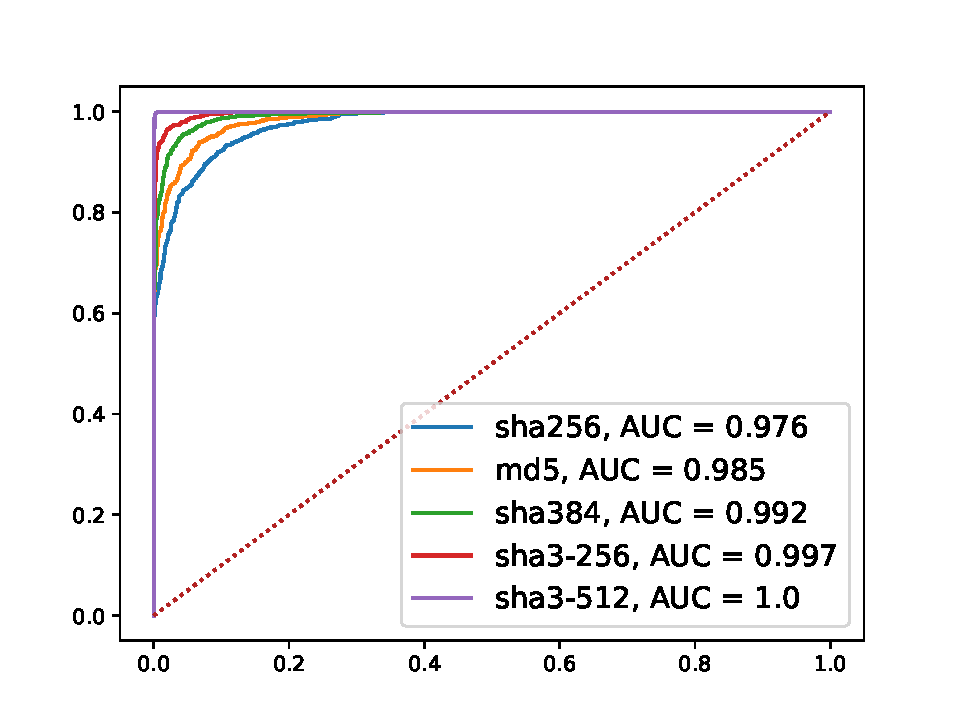
\includegraphics[width=\linewidth]{figures/lan_50_AdaBoost.pdf}
					\caption{Ada, lan}
				\end{subfigure}
				\begin{subfigure}{0.32\linewidth}
					\centering
					\includegraphics[width=\linewidth]{figures/lan_50_keras.pdf}
					\caption{CNN, lan}
				\end{subfigure}
				\begin{subfigure}{0.32\linewidth}
					\centering
					\includegraphics[width=\linewidth]{figures/wlan_50_AdaBoost.pdf}
					\caption{Ada, wlan}
				\end{subfigure}
				\begin{subfigure}{0.32\linewidth}
					\centering
					\includegraphics[width=\linewidth]{figures/8.8.8.8_50_AdaBoost.pdf}
					\caption{Ada, 8.8.8.8}
				\end{subfigure}
				\begin{subfigure}{0.32\linewidth}
					\centering
					\includegraphics[width=\linewidth]{figures/8.8.8.8_50_keras.pdf}
					\caption{CNN, 8.8.8.8}
				\end{subfigure}
				\begin{subfigure}{0.32\linewidth}
					\centering
					\includegraphics[width=\linewidth]{figures/wlan_50_keras.pdf}
					\caption{CNN, wlan}
				\end{subfigure}
				\begin{subfigure}{0.32\linewidth}
					\centering
					\includegraphics[width=\linewidth]{figures/81.92.228.153_50_AdaBoost.pdf}
					\caption{Ada, 81.92.228.153}
				\end{subfigure}
				\begin{subfigure}{0.32\linewidth}
					\centering
					\includegraphics[width=\linewidth]{figures/81.92.228.153_50_keras.pdf}
					\caption{CNN, 81.92.228.153}
				\end{subfigure}
				\begin{subfigure}{0.32\linewidth}
					\centering
					\includegraphics[width=\linewidth]{figures/66.211.175.229_50_AdaBoost.pdf}
					\caption{Ada, 66.211.175.229}
				\end{subfigure}
				\begin{subfigure}{0.32\linewidth}
					\centering
					\includegraphics[width=\linewidth]{figures/139.130.4.5_50_AdaBoost.pdf}
					\caption{Ada, 139.130.4.5}
				\end{subfigure}
				\begin{subfigure}{0.32\linewidth}
					\centering
					\includegraphics[width=\linewidth]{figures/139.130.4.5_50_keras.pdf}
					\caption{CNN, 139.130.4.5}
				\end{subfigure}
				\begin{subfigure}{0.32\linewidth}
					\centering
					\includegraphics[width=\linewidth]{figures/66.211.175.229_50_keras.pdf}
					\caption{CNN, 66.211.175.229}
				\end{subfigure}
			\begin{subfigure}{0.32\linewidth}
				\hphantom{a}
			\end{subfigure}
			\caption{Receiver operating characteristic curves (TPR against TNR) for the specific detection of hash-chain covert channels using different hash algorithms by means of AdaBoost models and convolutional neural networks for window size 50}
			\label{hash-roc}
			\end{figure}
		%
			\begin{figure}
				\begin{subfigure}{0.32\linewidth}
					\centering
					\includegraphics[width=\linewidth]{figures/md5_lan_AdaBoost.pdf}
					\caption{Ada, lan}
				\end{subfigure}
				\begin{subfigure}{0.32\linewidth}
					\centering
					\includegraphics[width=\linewidth]{figures/md5_lan_keras.pdf}
					\caption{CNN, lan}
				\end{subfigure}
				\begin{subfigure}{0.32\linewidth}
					\centering
					\includegraphics[width=\linewidth]{figures/md5_wlan_AdaBoost.pdf}
					\caption{Ada, wlan}
				\end{subfigure}
				\begin{subfigure}{0.32\linewidth}
					\centering
					\includegraphics[width=\linewidth]{figures/md5_8.8.8.8_AdaBoost.pdf}
					\caption{Ada, 8.8.8.8}
				\end{subfigure}
				\begin{subfigure}{0.32\linewidth}
					\centering
					\includegraphics[width=\linewidth]{figures/md5_8.8.8.8_keras.pdf}
					\caption{CNN, 8.8.8.8}
				\end{subfigure}
				\begin{subfigure}{0.32\linewidth}
					\centering
					\includegraphics[width=\linewidth]{figures/md5_wlan_keras.pdf}
					\caption{CNN, wlan}
				\end{subfigure}
				\begin{subfigure}{0.32\linewidth}
					\centering
					\includegraphics[width=\linewidth]{figures/md5_81.92.228.153_AdaBoost.pdf}
					\caption{Ada, 81.92.228.153}
				\end{subfigure}
				\begin{subfigure}{0.32\linewidth}
					\centering
					\includegraphics[width=\linewidth]{figures/md5_81.92.228.153_keras.pdf}
					\caption{CNN, 81.92.228.153}
				\end{subfigure}
				\begin{subfigure}{0.32\linewidth}
					\centering
					\includegraphics[width=\linewidth]{figures/md5_66.211.175.229_AdaBoost.pdf}
					\caption{Ada, 66.211.175.229}
				\end{subfigure}
				\begin{subfigure}{0.32\linewidth}
					\centering
					\includegraphics[width=\linewidth]{figures/md5_139.130.4.5_AdaBoost.pdf}
					\caption{Ada, 139.130.4.5}
				\end{subfigure}
				\begin{subfigure}{0.32\linewidth}
					\centering
					\includegraphics[width=\linewidth]{figures/md5_139.130.4.5_keras.pdf}
					\caption{CNN, 139.130.4.5}
				\end{subfigure}
				\begin{subfigure}{0.32\linewidth}
				\centering
				\includegraphics[width=\linewidth]{figures/md5_66.211.175.229_keras.pdf}
				\caption{CNN, 66.211.175.229}
				\end{subfigure}
			\begin{subfigure}{0.32\linewidth}
				\hphantom{a}
			\end{subfigure}
				\caption{Receiver operating characteristic curves (TPR against TNR) for the specific  detection of md5 hash-chain covert channels using different window sizes by means of AdaBoost models and convolutional neural networks}
				\label{window-roc}
			\end{figure}
			The performances of both approaches are remarkably similar, as can be seen by the ROC curves in figures \ref{hash-roc} and \ref{window-roc}. In general, the ability for detection increases with higher hash-runtime and greater window sizes. For high latency connections the ability of the convolutional neural network to detect covert channels using the higher runtime sha3-256 and sha3-512 hashes is sometimes lower than for the other hashes (c.f. figure \ref{stat-mes-fig} (k)), which can be explained by random chance due to the less significant difference between modified and unmodified traffic for higher latency connections. \\
			We confirmed our results through the application of select statistical models on real covert traffic provided by Schmidbauer and Wendzel  \cite{Schmidbauer}. We sampled sets of window size 50, split them into training and validation data and used the training data to train our models. Figure \ref{Schm-perf} shows the AUC scores for the mean-threshold detection developed in \cite{Schmidbauer} as well as the AdaBoost and convolutional neural network approaches for the four physically implemented covert channels using the optimal alphabet with the sha384, md5, sha3-256 and sha3-512 hashes. Both of our models are able to successfully detect the covert channel's presence with the convolutional neural network performing the best. In contrast to the data reported in figure \ref{hash-roc}, no clear relationship between hash runtime and detectability can be observed, which could be explained by the high latency present in the measurements similar to the behaviour observed in figure \ref{stat-mes-fig} (k).\\
			Schmidbauer and Wendzel performed their mean-threshold test on 5000 packet measurements to predict whether or not a covert channel was present. For sha384, md5 and sha3-256 both AdaBoost and convolutional neural network classification achieve significantly higher AUC scores while using only 50 measurements. With the high runtime sha3-512 hash, the mean-threshold detection from \cite{Schmidbauer} outperforms the detection via CNN and AdaBoost, however considering the smaller measurement size the comparable performance of the convolutional neural network and the mean-threshold test using 5000 measurements is still impressive.
			\begin{figure}
				\centering
				\includegraphics[width=0.75\linewidth]{figures/native.pdf}
				\caption{Comparison of selected statistical models on the covert channel dataset investigated in \cite{Schmidbauer}. Schmidbauer and Wendzel used mean-threshold detection on sets of 5000 measurements. Ada and CNN models used window size 50.}
				\label{Schm-perf}
			\end{figure}
		
		
	%---------------------------------------------------------
	%						Conclusion
	%---------------------------------------------------------
	\chapter{Conclusion}
	
			Throughout this thesis we argued for the detectability of computationally intensive covert channels with shape analysis of packet runtime empirical probability distributions. We provided evidence both for the existence of singular metrics that could be used in this task, such as the Süssmann measure, as well as the efficacy of statistical models and neural networks in improving detection accuracy. \\
			Qualitative analysis of traffic flows was used to indicate a significant and detectable shape difference between modified and regular traffic flow for the studied hash-chain covert channel. Based on this observation a number of statistical measures were investigated for their potential to indicate this difference with mixed results. Machine learning models trained on this collection of statistical measures showed great success with tree models being particularly well suited for the task of covert channel detection. Lastly a direct application of convolutional neural networks to the empirical probability density function of packet runtimes was tested and shown to possess great potential to recognise shape differences even based on minimal data. The efficacy of the most promising models has been further confirmed by training and testing them on traffic measurements taken from a physical implementation of the investigated channel. \\
			This work provides evidence for the general detectability of reversible covert channels, the potential of runtime distribution shape analysis for network anomaly detection and the applicability of convolutional neural networks to this task. While our methodology allows for significant improvements of covert channel detection accuracy for higher latency connections, it also further underlines the observation made in  \cite{Schmidbauer} that detectability of reversible covert traffic is inversely correlated to the latency and hop count of a connection.\\
			Further research still needs to be done on the applicability of shape analysis in real world scenarios. Robustness against concept drift and the ability to adapt to different types of covert channels need to be demonstrated. For an anomaly detection model to be useful it needs to be able to differentiate natural concept drifts from various malicious activities. The investigated covert channel runtime distribution can be modified by varying the alphabet used to communicate and using traffic normalization. Neither of these possibilities are accounted for in thesis. Potential for research also lies in the generalizability of shape analysis to enable relative detection on multiple connections with a singular statistical model. \\ 
			While this detection approach still requires more work to be done in order to be reliably implemented, probability distribution shape analysis could prove to be a valuable tool when dealing with reversible covert channels.
			
	
	%---------------------------------------------------------
	%						Bibliography
	%---------------------------------------------------------
	\pagebreak
	
	\pagenumbering{Roman}
	\printbibliography
	
\end{document}